\section{Bertrand pricing with logit demand: single- and multi-product firms}\label{sec:C-logit-bertrand}

The first two problems treated a homogeneous good, where one price clears the market and conduct is summarized by
a single parameter. From here on products are differentiated, firms set prices, and substitution between products
governs market power. The logit model is the simplest demand system for differentiated products in which
Bertrand-Nash prices have closed forms. This problem uses it to compute price equilibria, to show how joint ownership of several products
raises prices, and to prove that the equilibrium is unique. Two further parts evaluate a merger and a common unit
tax. The market is the 25-product market of \cref{ex:04-logit25}, and the theory is that of \cref{ch:diffprod}. We
restate each result we use and prove the ones that \cref{ch:diffprod} leaves open.

\subsection{Statement}

A single market has a unit mass of consumers, 25 inside products and an outside good. Consumer $i$ obtains utility
$u_{ij} = \delta_j + \epsilon_{ij}$ from product $j$ and $u_{i0} = \epsilon_{i0}$ from the outside good, where the
$\epsilon_{ij}$ are independent type-I extreme value shocks. The mean utility of product $j$ is
\begin{equation}\label{eq:C-logit-delta}
  \delta_j = x_j\beta - \alpha p_j + \xi_j , \qquad x_j = (1, x_{2j}, x_{3j}) ,
\end{equation}
where $x_{2j}$ is a continuous characteristic, $x_{3j}$ is a binary characteristic and $\xi_j$ is quality that
the econometrician does not observe. Marginal cost is constant and equal to
\begin{equation}\label{eq:C-logit-mc}
  mc_j = x_j\gamma + \omega_j .
\end{equation}
The parameters are $\beta = (0.1, 0.25, 0.1)$, $\alpha = 2$ and $\gamma = (0.2, 0.25, 0.3)$.
\Cref{tab:C-logit-data} lists the characteristics, the shocks and the implied marginal costs. The continuous
characteristic has mean 1.79, standard deviation 1.02 and range $-0.006$ to 4.18. Eleven products have $x_{3j} = 1$.
The quality shocks have mean 0.195 and standard deviation 1.00. The cost shocks have mean $-0.013$ and standard
deviation 0.045, and marginal costs range from 0.164 to 1.236. Five owners, labeled 0 to 4, hold 3, 3, 6, 6 and 7
products. Product labels 0 to 24 are names. The symbol $s_0$ always denotes the share of the outside good.

Firms know all characteristics, shocks and parameters, so the game has complete information. They set prices
simultaneously.

\begin{table}[htbp]
\centering
\caption{Product characteristics, shocks and marginal costs in the 25-product logit market}
\label{tab:C-logit-data}
\footnotesize
\setlength{\tabcolsep}{4pt}
\begin{tabular}{@{}rrrrrrr@{\hspace{14pt}}rrrrrrr@{}}
\toprule
$j$ & owner & $x_{2j}$ & $x_{3j}$ & $\xi_j$ & $\omega_j$ & $mc_j$ &
$j$ & owner & $x_{2j}$ & $x_{3j}$ & $\xi_j$ & $\omega_j$ & $mc_j$ \\
\midrule
0 & 2 & 1.277 & 1 & 0.158 & $-0.030$ & 0.790 & 13 & 3 & 1.582 & 1 & 0.167 & $-0.044$ & 0.852 \\
1 & 4 & 2.310 & 1 & 0.545 & 0.021 & 1.099 & 14 & 3 & 2.141 & 0 & 0.027 & $-0.057$ & 0.678 \\
2 & 3 & 1.942 & 0 & $-0.342$ & 0.003 & 0.689 & 15 & 3 & 0.915 & 0 & 0.317 & 0.024 & 0.453 \\
3 & 2 & 2.464 & 1 & 1.085 & 0.031 & 1.147 & 16 & 2 & 3.066 & 0 & 0.880 & 0.010 & 0.977 \\
4 & 2 & $-0.006$ & 0 & $-0.235$ & $-0.034$ & 0.164 & 17 & 3 & 0.155 & 1 & 0.576 & $-0.021$ & 0.517 \\
5 & 0 & 1.243 & 1 & 1.943 & $-0.056$ & 0.755 & 18 & 4 & 1.025 & 1 & 1.073 & 0.030 & 0.786 \\
6 & 2 & 2.675 & 0 & $-1.296$ & $-0.031$ & 0.838 & 19 & 3 & 1.280 & 1 & 1.613 & $-0.097$ & 0.724 \\
7 & 4 & 2.141 & 0 & $-1.418$ & $-0.041$ & 0.695 & 20 & 4 & 1.107 & 1 & 2.047 & $-0.001$ & 0.776 \\
8 & 2 & 1.998 & 0 & $-1.552$ & 0.036 & 0.735 & 21 & 0 & 4.183 & 0 & $-0.911$ & $-0.010$ & 1.236 \\
9 & 4 & 0.902 & 0 & $-1.122$ & 0.025 & 0.450 & 22 & 4 & 1.545 & 1 & 0.206 & 0.039 & 0.925 \\
10 & 1 & 3.795 & 0 & $-0.247$ & $-0.098$ & 1.050 & 23 & 0 & 2.044 & 0 & 1.019 & $-0.052$ & 0.659 \\
11 & 1 & 2.925 & 0 & 0.179 & 0.059 & 0.991 & 24 & 1 & 0.861 & 1 & $-0.618$ & 0.038 & 0.753 \\
12 & 4 & 1.232 & 0 & 0.772 & $-0.081$ & 0.427 & & & & & & & \\
\bottomrule
\end{tabular}

\vspace{3pt}
\begin{minipage}{0.97\textwidth}
\footnotesize Notes: Every product also has the constant characteristic $x_{1j} = 1$. Marginal cost is
$mc_j = x_j\gamma + \omega_j$ with $\gamma = (0.2, 0.25, 0.3)$. Owners 0 to 4 hold products $\{5, 21, 23\}$,
$\{10, 11, 24\}$, $\{0, 3, 4, 6, 8, 16\}$, $\{2, 13, 14, 15, 17, 19\}$ and $\{1, 7, 9, 12, 18, 20, 22\}$. Values
rounded to three decimals.
\end{minipage}
\end{table}

\begin{enumerate}[label=(\alph*)]
  \item Suppose that every product is sold by a separate firm. Derive the market shares, the profits and the
  derivatives of the shares with respect to prices. State the own- and cross-price elasticities.
  \item Derive the best-response price of product $j$ to the prices of the other products. Show that it is the
  unique maximizer of the firm's profit.
  \item Define a Nash equilibrium of the pricing game.
  \item Describe three algorithms that compute the equilibrium. Implement one of them and report prices, markups,
  shares, profits and consumer surplus.
  \item Now each owner in \cref{tab:C-logit-data} sets the prices of all its products jointly. Repeat parts (a) to
  (d), compare the two equilibria and explain the differences.
  \item Is each equilibrium unique? Prove your answer and verify it numerically.
  \item Owners 3 and 4 merge. Compute the post-merger equilibrium. Compare the price changes with the upward
  pricing pressure that the merger creates at pre-merger prices.
  \item A unit tax $t$ is added to the marginal cost of every product. Derive the pass-through of a cost increase to
  the prices of one firm, holding rivals' prices fixed. Derive the equilibrium pass-through of the common tax,
  compute it for $t = 0.1$, and compute the pass-through of the share-weighted average price.
\end{enumerate}

\subsection{Solution}

\casehead{Part (a)}
Write $a_j = x_j\beta + \xi_j$ for the part of mean utility that does not depend on price, so that
$\delta_j = a_j - \alpha p_j$. The mean utility of the outside good is normalized to zero. Let
\begin{equation}\label{eq:C-logit-Phi}
  \Phi = 1 + \sum_{l=0}^{24} e^{\delta_l}
\end{equation}
be the logit denominator, where the 1 is the outside good's contribution $e^0$. The extreme value shocks give the
logit choice probabilities (\cref{ch:discrete}). With a unit mass of consumers, shares equal quantities:
\begin{equation}\label{eq:C-logit-shares}
  s_j(p) = \frac{e^{\delta_j}}{\Phi} , \qquad s_0(p) = \frac{1}{\Phi} .
\end{equation}
A firm $f$ that owns the set of products $\mathcal{J}_f$ earns
\begin{equation}\label{eq:C-logit-profit}
  \pi_f(p) = \sum_{k \in \mathcal{J}_f}(p_k - mc_k)\,s_k(p) .
\end{equation}
With single-product firms, $\mathcal{J}_f = \{j\}$ and $\pi_j(p) = (p_j - mc_j)s_j(p)$.

A change in $p_j$ moves the numerator of $s_j$ and the denominator $\Phi$ at the same rate,
$\frac{\partial e^{\delta_j}}{\partial p_j} = \frac{\partial\Phi}{\partial p_j} = -\alpha e^{\delta_j}$. The quotient rule gives
\begin{equation*}
  \frac{\partial s_j}{\partial p_j}
  = \frac{-\alpha e^{\delta_j}\Phi + \alpha e^{\delta_j}e^{\delta_j}}{\Phi^2}
  = -\alpha s_j + \alpha s_j^2
  = -\alpha s_j(1 - s_j) .
\end{equation*}
For $k \ne j$, including the outside good, only the denominator of $s_k$ depends on $p_j$, so
\begin{equation*}
  \frac{\partial s_k}{\partial p_j} = -\frac{e^{\delta_k}}{\Phi^2}\,\frac{\partial\Phi}{\partial p_j}
  = \frac{\alpha e^{\delta_k}e^{\delta_j}}{\Phi^2} = \alpha s_js_k .
\end{equation*}
These are the derivatives in \eqref{eq:04-logit-derivs}. Let $\Delta$ be the $25 \times 25$ matrix with
$\Delta_{jk} = \frac{\partial s_j}{\partial p_k}$. Then
\begin{equation}\label{eq:C-logit-Delta}
  \Delta = \alpha\big(ss^\top - \diag(s)\big) ,
\end{equation}
which is symmetric. We write elasticities as $\varepsilon_{jk} = \frac{\partial s_j}{\partial p_k}\frac{p_k}{s_j}$,
so own elasticities are negative. The positive own elasticity of the notation list is $-\varepsilon_{jj}$. Then
\begin{equation}\label{eq:C-logit-elast}
  \varepsilon_{jj} = -\alpha p_j(1 - s_j) , \qquad \varepsilon_{jk} = \alpha p_ks_k \quad (k \ne j) .
\end{equation}
The cross elasticity with respect to $p_k$ is the same for every $j \ne k$. This is the independence of irrelevant
alternatives (\cref{ch:logit}). Own elasticities are roughly proportional to price, because shares are small.

\casehead{Part (b)}
Firm $j$ chooses $p_j$ to maximize $\pi_j$ given the rival prices $p_{-j}$. Let $m_j = p_j - mc_j$ denote the
markup. By part (a),
\begin{equation}\label{eq:C-logit-dpi}
  \frac{\partial\pi_j}{\partial p_j} = s_j + m_j\frac{\partial s_j}{\partial p_j} = s_j\big[1 - \alpha m_j(1 - s_j)\big] .
\end{equation}
Since $s_j > 0$, the first-order condition is
\begin{equation}\label{eq:C-logit-markup-single}
  m_j = \frac{1}{\alpha(1 - s_j)} .
\end{equation}
The condition is implicit, because $s_j$ depends on $p_j$. To solve it, separate the part of $\Phi$ that firm $j$
controls. Let $v_j = a_j - \alpha\,mc_j$ be the mean utility of product $j$ when it is priced at marginal cost, so
that $\delta_j = v_j - \alpha m_j$. Let $\Phi_{-j} = 1 + \sum_{l \ne j}e^{\delta_l}$, which depends only on rival
prices. Then $\Phi = \Phi_{-j} + e^{\delta_j}$ and $1 - s_j = \frac{\Phi_{-j}}{\Phi_{-j} + e^{\delta_j}}$. Substitute this
into \eqref{eq:C-logit-markup-single} and multiply both sides by $\Phi_{-j} + e^{\delta_j}$:
\begin{align*}
  \alpha m_j\Phi_{-j} &= \Phi_{-j} + e^{v_j - \alpha m_j} , \\
  (\alpha m_j - 1)\Phi_{-j} &= e^{v_j - \alpha m_j} .
\end{align*}
Multiply both sides by $\frac{e^{\alpha m_j - 1}}{\Phi_{-j}}$:
\begin{equation}\label{eq:C-lambert-eq}
  (\alpha m_j - 1)\,e^{\alpha m_j - 1} = \frac{e^{v_j - 1}}{\Phi_{-j}} .
\end{equation}
The left side has the form $we^w$ with $w = \alpha m_j - 1$. The next lemma inverts it.

\begin{lemma}[Lambert W function]\label{lem:C-lambert}
For every $z > 0$ the equation $we^w = z$ has exactly one real solution, denoted $W(z)$, and $W(z) > 0$. The
function $W$ is differentiable and strictly increasing on $(0, \infty)$, with
\begin{equation}\label{eq:C-lambert-deriv}
  W'(z) = \frac{W(z)}{z\,\big(1 + W(z)\big)} .
\end{equation}
The ratio $\frac{W(z)}{1 + W(z)}$ is strictly increasing in $z$ and lies in $(0, 1)$.
\end{lemma}

\begin{proof}
Let $g(w) = we^w$. If $w \le 0$, then $g(w) \le 0 < z$, so no solution is negative or zero. On $(0, \infty)$,
$g'(w) = (1 + w)e^w > 0$, $g(0) = 0$ and $g(w) \to \infty$. By continuity and strict monotonicity, $g(w) = z$ has
exactly one solution, and it is positive. The inverse function theorem gives
$W'(z) = \frac{1}{g'(W(z))} = \frac{1}{(1 + W)e^W}$. Since $e^W = \frac{z}{W}$, this equals
\eqref{eq:C-lambert-deriv}, which is positive. Finally $\frac{W}{1 + W} = 1 - \frac{1}{1 + W}$ rises with $W$, and
$W$ rises with $z$.
\end{proof}

The function $W$ is the principal branch of the Lambert W function \citep{CorlessEtAl1996}. Applying
\cref{lem:C-lambert} with $z = \frac{e^{v_j - 1}}{\Phi_{-j}} > 0$ to \eqref{eq:C-lambert-eq} gives the best response
\begin{equation}\label{eq:C-br-single}
  BR_j(p_{-j}) = mc_j + \frac{1}{\alpha}\Big[1 + W\Big(\frac{e^{v_j - 1}}{\Phi_{-j}}\Big)\Big] .
\end{equation}
This is \eqref{eq:04-logit-br}. Three properties follow at once. The best-response markup exceeds $\frac{1}{\alpha}$,
because $W > 0$. It rises with $v_j$, the product's quality net of cost. It rises with every rival price, because a
higher $p_l$ lowers $\Phi_{-j}$ and $W$ is increasing. Prices are strategic complements.

The stationary point is the unique global maximizer. Write \eqref{eq:C-logit-dpi} as $s_j\,G(m_j)$ with
$G(m) = 1 - \alpha m\,(1 - s_j)$, where $s_j$ is evaluated at $p_j = mc_j + m$. If $m \le 0$, then $G(m) \ge 1$ and
profit rises with the price. If $m > 0$, both $\alpha m$ and $1 - s_j$ are positive and strictly increasing in $m$,
because $s_j$ falls as $p_j$ rises. So $G$ is strictly decreasing on $(0, \infty)$, and $G(m) \to -\infty$ because
$1 - s_j \to 1$. Hence $G$ has exactly one zero. Profit rises below it and falls above it, and
\eqref{eq:C-br-single} is the unique maximizer of $\pi_j$.

\casehead{Part (c)}
The players are the 25 firms. Firm $j$ chooses $p_j \in \R$ and receives $\pi_j(p_j, p_{-j})$. A \emph{Nash
equilibrium} is a price vector $p^*$ such that
\begin{equation*}
  \pi_j(p_j^*, p_{-j}^*) \ge \pi_j(p_j, p_{-j}^*) \qquad \text{for every } p_j \in \R \text{ and every } j .
\end{equation*}
Equivalently, $p^* = BR(p^*)$, where $BR(p) = \big(BR_0(p_{-0}), \dots, BR_{24}(p_{-24})\big)$ is the best-response
map. By part (b), each best response is unique and solves the first-order condition, so $p^*$ is an equilibrium if
and only if
\begin{equation}\label{eq:C-foc-single}
  s_j(p^*) + (p_j^* - mc_j)\frac{\partial s_j}{\partial p_j}(p^*) = 0 , \qquad j = 0, \dots, 24 .
\end{equation}
Complete information matters here. Each best response depends on $\Phi_{-j}$, which requires every rival's price
and mean utility.

\casehead{Part (d)}
Three algorithms are standard.
\begin{enumerate}
  \item \emph{Best-response iteration.} Start from $p^{(0)} = mc + \frac{1}{\alpha}$, the markup that
  \eqref{eq:C-logit-markup-single} gives when shares are negligible. Set $p^{(n+1)} = BR(p^{(n)})$ with
  \eqref{eq:C-br-single}, and stop when $\|p^{(n+1)} - p^{(n)}\|_\infty < 10^{-12}$. Part (f) shows that the
  iteration converges from any starting point.
  \item \emph{Markup iteration.} Iterate on the first-order condition itself,
  $p^{(n+1)} = mc + \frac{1}{\alpha(1 - s(p^{(n)}))}$, element by element. The method needs no special function,
  but nothing guarantees its convergence in general.
  \item \emph{Newton-type root finding.} Solve the 25 equations \eqref{eq:C-foc-single} with a quasi-Newton
  method. We use the hybrid Powell method with tolerance $10^{-14}$, started at $mc + \frac{1}{\alpha}$.
\end{enumerate}
Best-response iteration converges in 10 iterations, markup iteration in 14, and the root finder uses 39 function
evaluations. The three solutions agree to within $1.2\times10^{-14}$, and the largest first-order residual is
$1.5\times10^{-15}$.

The columns marked S in \cref{tab:C-logit-eq} report the equilibrium. Markups range from 0.502 to 0.566. They lie
close to the floor $\frac{1}{\alpha} = 0.5$, because every share is small, and they rise with the share, as
\eqref{eq:C-logit-markup-single} requires. Products 20 and 5, with shares of 11.66 and 11.37 percent, carry the
largest markups, 0.566 and 0.564. The outside good takes 13.67 percent of the market, so $\Phi^* = \frac{1}{s_0} = 7.314$.
Total profit is 0.4616, and the share-weighted mean price is 1.2599.

Consumer surplus follows from the log-sum formula of \cref{sec:06-logsum} \citep{SmallRosen1981}. The expected
maximum utility is $\E[\max_{j}u_{ij}] = \ln\Phi + \gamma_E$, where $\gamma_E \approx 0.5772$ is Euler's constant.
Dividing by the marginal utility of money $\alpha$ converts utility into money. Consumer surplus per consumer is
therefore $\frac{1}{\alpha}\ln\Phi$ up to an additive constant, which equals 0.9949 here. Only differences in
consumer surplus across scenarios have meaning.

\casehead{Part (e)}
Firm $f$ now chooses all prices in $\mathcal{J}_f$ to maximize \eqref{eq:C-logit-profit}. For $j \in \mathcal{J}_f$, the
derivatives of part (a) give
\begin{align*}
  \frac{\partial\pi_f}{\partial p_j}
  &= s_j + \sum_{k \in \mathcal{J}_f}m_k\frac{\partial s_k}{\partial p_j} \\
  &= s_j - \alpha m_js_j(1 - s_j) + \sum_{k \in \mathcal{J}_f,\, k \ne j}\alpha m_ks_js_k \\
  &= s_j\Big[1 - \alpha m_j + \alpha\sum_{k \in \mathcal{J}_f}m_ks_k\Big] .
\end{align*}
Setting the derivative to zero and dividing by $\alpha s_j > 0$ gives
\begin{equation}\label{eq:C-mp-foc}
  m_j = \frac{1}{\alpha} + \sum_{k \in \mathcal{J}_f}s_km_k \qquad \text{for every } j \in \mathcal{J}_f .
\end{equation}

\begin{proposition}[Common markup]\label{prop:C-common-markup}
At any price vector at which firm $f$'s first-order conditions hold, all products of $f$ carry the same markup
\begin{equation}\label{eq:C-common-markup}
  m_f = \frac{1}{\alpha(1 - S_f)} , \qquad S_f = \sum_{k \in \mathcal{J}_f}s_k .
\end{equation}
\end{proposition}

This is \cref{prop:04-logit-markup}. It follows from \eqref{eq:C-mp-foc}, whose right side does not depend on $j$. The
firm prices as a single-product firm whose share is its combined share.
Quality and cost differences among its products move their prices one for one with cost and affect markups only
through $S_f$. Dividing \eqref{eq:C-mp-foc} by $1 - s_j$ gives a second reading,
\begin{equation}\label{eq:C-mp-foc-diversion}
  m_j = \frac{1}{\alpha(1 - s_j)} + \sum_{k \in \mathcal{J}_f,\, k \ne j}D_{jk}m_k ,
  \qquad D_{jk} = -\frac{\partial s_k}{\partial p_j}\Big(\frac{\partial s_j}{\partial p_j}\Big)^{-1} = \frac{s_k}{1 - s_j} .
\end{equation}
The markup of product $j$ equals its single-product markup plus the margin earned on the sales that a price increase
diverts to the firm's other products. $D_{jk}$ is the logit \emph{diversion ratio} from $j$ to $k$, the fraction of the sales lost by $j$ that go to $k$.

The multi-product best response follows the steps of part (b). Let $E_f = \sum_{k \in \mathcal{J}_f}e^{v_k}$ and
$\Phi_{-f} = 1 + \sum_{l \notin \mathcal{J}_f}e^{\delta_l}$, which depends only on rivals' prices. At a common markup
$m$, firm $f$'s products contribute $\sum_{k \in \mathcal{J}_f}e^{v_k - \alpha m} = E_fe^{-\alpha m}$ to $\Phi$, so
\begin{equation*}
  S_f = \frac{E_fe^{-\alpha m}}{\Phi_{-f} + E_fe^{-\alpha m}} , \qquad
  1 - S_f = \frac{\Phi_{-f}}{\Phi_{-f} + E_fe^{-\alpha m}} .
\end{equation*}
Substitute $1 - S_f$ into $\alpha m(1 - S_f) = 1$ and clear the denominator:
\begin{align*}
  \alpha m\,\Phi_{-f} &= \Phi_{-f} + E_fe^{-\alpha m} , \\
  (\alpha m - 1)\Phi_{-f} &= E_fe^{-\alpha m} , \\
  (\alpha m - 1)e^{\alpha m - 1} &= \frac{E_fe^{-1}}{\Phi_{-f}} ,
\end{align*}
where the last line multiplies by $\frac{e^{\alpha m - 1}}{\Phi_{-f}}$. \Cref{lem:C-lambert} gives
\begin{equation}\label{eq:C-br-multi}
  m_f^{BR} = \frac{1}{\alpha}\Big[1 + W\Big(\frac{E_fe^{-1}}{\Phi_{-f}}\Big)\Big] , \qquad
  BR_k(p_{-\mathcal{J}_f}) = mc_k + m_f^{BR} \quad (k \in \mathcal{J}_f) .
\end{equation}
With one product, $E_f = e^{v_j}$ and \eqref{eq:C-br-multi} reduces to \eqref{eq:C-br-single}. \Cref{ch:diffprod}
states this formula, \eqref{eq:04-logit-br-multi}, and proves its global optimality in Steps 1 and 2 of the proof
of \cref{thm:04-logit-unique}. The next proposition gives a second proof, by a change of variables from prices to
shares under which profit is concave.

\begin{proposition}[Profit is concave in shares]\label{prop:C-firm-concave}
Fix the rivals' prices, and hence $\Phi_{-f}$.
\begin{enumerate}[label=(\roman*)]
  \item The map from firm $f$'s prices $(p_k)_{k \in \mathcal{J}_f}$ to its shares $(s_k)_{k \in \mathcal{J}_f}$ is a
  smooth bijection onto $\{s > 0 : S_f < 1\}$, with smooth inverse
  \begin{equation}\label{eq:C-share-inverse}
    \delta_k = \ln s_k + \ln\Phi_{-f} - \ln(1 - S_f) .
  \end{equation}
  \item As a function of its shares, firm $f$'s profit is
  \begin{equation}\label{eq:C-profit-shares}
    \pi_f = \frac{1}{\alpha}\sum_{k \in \mathcal{J}_f}s_k\big[v_k - \ln\Phi_{-f} - \ln s_k\big] + \frac{1}{\alpha}S_f\ln(1 - S_f) ,
  \end{equation}
  which is strictly concave.
  \item Profit has a unique maximizer over $f$'s prices. It is the unique solution of $f$'s first-order
  conditions and is given by \eqref{eq:C-br-multi}.
\end{enumerate}
\end{proposition}

\begin{proof}
(i) Given prices, shares follow from \eqref{eq:C-logit-shares}. Conversely, take shares with $s_k > 0$ and $S_f < 1$.
Because $\Phi = \Phi_{-f} + \sum_{k \in \mathcal{J}_f}e^{\delta_k} = \Phi_{-f} + S_f\Phi$, the denominator must equal
$\Phi = \frac{\Phi_{-f}}{1 - S_f}$. Then $e^{\delta_k} = s_k\Phi$ gives \eqref{eq:C-share-inverse}, and
$p_k = \frac{a_k - \delta_k}{\alpha}$. Both maps are smooth, and they are inverse to each other.

(ii) The markup is $m_k = p_k - mc_k = \frac{a_k - \delta_k}{\alpha} - mc_k = \frac{v_k - \delta_k}{\alpha}$.
Substituting \eqref{eq:C-share-inverse},
\begin{equation*}
  \alpha m_k = v_k - \ln s_k - \ln\Phi_{-f} + \ln(1 - S_f) .
\end{equation*}
Multiplying by $\frac{s_k}{\alpha}$ and summing over $k \in \mathcal{J}_f$ gives \eqref{eq:C-profit-shares}. In the first
sum, each term is linear in $s_k$ except $-s_k\ln s_k$, whose second derivative is $-\frac{1}{s_k} < 0$. In the second
term, $\varphi(S) = S\ln(1 - S)$ has
\begin{equation*}
  \varphi'(S) = \ln(1 - S) - \frac{S}{1 - S} , \qquad
  \varphi''(S) = -\frac{1}{1 - S} - \frac{1}{(1 - S)^2} < 0 ,
\end{equation*}
and $S_f$ is linear in the shares. A sum of strictly concave functions of separate shares and a concave function of
their sum is strictly concave.

(iii) The partial derivative of \eqref{eq:C-profit-shares} is
\begin{equation*}
  \frac{\partial\pi_f}{\partial s_k} = \frac{1}{\alpha}\big[v_k - \ln\Phi_{-f} - \ln s_k - 1 + \varphi'(S_f)\big] .
\end{equation*}
It tends to $+\infty$ as $s_k \to 0$ with $S_f$ bounded away from one, and profit tends to $-\infty$ as
$S_f \to 1$. A maximizer therefore exists and is interior, and strict concavity makes it the only stationary point.
By (i), stationary points in prices and in shares coincide, because the change of variables has an invertible
Jacobian. By \cref{prop:C-common-markup} and the derivation above, the only stationary point in prices is
\eqref{eq:C-br-multi}.
\end{proof}

Stacking the first-order conditions of all firms gives one system for any ownership structure. Let $\Omega$ be the
ownership matrix, with $\Omega_{jk} = 1$ when $j$ and $k$ have the same owner and zero otherwise. The condition
for $p_j$ is $s_j + \sum_k\Omega_{jk}\frac{\partial s_k}{\partial p_j}m_k = 0$. Since
$\frac{\partial s_k}{\partial p_j} = \Delta_{kj}$, in matrix form
\begin{equation}\label{eq:C-stacked-foc}
  s + (\Omega \odot \Delta^\top)(p - mc) = 0 ,
\end{equation}
with $\odot$ the element-wise product. Single-product firms correspond to $\Omega = I$. Only $\Omega$ changes between
the two games, so a program written for \eqref{eq:C-stacked-foc} handles both.

All three algorithms of part (d) carry over. Best-response iteration now uses \eqref{eq:C-br-multi}. Markup
iteration uses $p^{(n+1)}_k = mc_k + \frac{1}{\alpha(1 - S_f(p^{(n)}))}$. Best-response iteration converges in 15
iterations, markup iteration in 30, and the root finder uses 41 function evaluations. The solutions agree to within
$1.4\times10^{-13}$, and the largest first-order residual is $1.5\times10^{-14}$.

\begin{table}[htbp]
\centering
\caption{Equilibrium by product: single-product firms (S), five multi-product owners (M), and after the merger of
owners 3 and 4 (G)}
\label{tab:C-logit-eq}
\footnotesize
\setlength{\tabcolsep}{5pt}
\begin{tabular}{@{}rrrrrrrrrrr@{}}
\toprule
 & & & \multicolumn{3}{c}{Price} & \multicolumn{2}{c}{Markup} & \multicolumn{3}{c}{Share (\%)} \\
\cmidrule(lr){4-6}\cmidrule(lr){7-8}\cmidrule(l){9-11}
$j$ & owner & $mc_j$ & $p_j^S$ & $p_j^M$ & $p_j^G$ & $m_j^S$ & $m_j^M$ & $s_j^S$ & $s_j^M$ & $s_j^G$ \\
\midrule
0 & 2 & 0.790 & 1.300 & 1.369 & 1.382 & 0.510 & 0.579 & 2.00 & 2.04 & 2.32 \\
1 & 4 & 1.099 & 1.609 & 1.769 & 1.920 & 0.510 & 0.670 & 2.05 & 1.75 & 1.51 \\
2 & 3 & 0.689 & 1.197 & 1.325 & 1.510 & 0.508 & 0.636 & 1.59 & 1.44 & 1.16 \\
3 & 2 & 1.147 & 1.664 & 1.726 & 1.739 & 0.517 & 0.579 & 3.29 & 3.40 & 3.86 \\
4 & 2 & 0.164 & 0.680 & 0.744 & 0.757 & 0.516 & 0.579 & 3.06 & 3.16 & 3.59 \\
5 & 0 & 0.755 & 1.319 & 1.371 & 1.389 & 0.564 & 0.616 & 11.37 & 12.00 & 13.50 \\
6 & 2 & 0.838 & 1.341 & 1.418 & 1.430 & 0.503 & 0.579 & 0.55 & 0.55 & 0.63 \\
7 & 4 & 0.695 & 1.198 & 1.365 & 1.516 & 0.503 & 0.670 & 0.57 & 0.48 & 0.41 \\
8 & 2 & 0.735 & 1.237 & 1.314 & 1.327 & 0.502 & 0.579 & 0.44 & 0.45 & 0.51 \\
9 & 4 & 0.450 & 0.955 & 1.120 & 1.272 & 0.505 & 0.670 & 0.91 & 0.77 & 0.66 \\
10 & 1 & 1.050 & 1.557 & 1.575 & 1.579 & 0.507 & 0.524 & 1.35 & 1.53 & 1.77 \\
11 & 1 & 0.991 & 1.500 & 1.515 & 1.519 & 0.510 & 0.524 & 1.87 & 2.12 & 2.46 \\
12 & 4 & 0.427 & 0.962 & 1.097 & 1.248 & 0.535 & 0.670 & 6.50 & 5.81 & 5.01 \\
13 & 3 & 0.852 & 1.362 & 1.488 & 1.673 & 0.510 & 0.636 & 1.92 & 1.75 & 1.41 \\
14 & 3 & 0.678 & 1.191 & 1.315 & 1.500 & 0.513 & 0.636 & 2.45 & 2.24 & 1.81 \\
15 & 3 & 0.453 & 0.972 & 1.089 & 1.274 & 0.519 & 0.636 & 3.73 & 3.46 & 2.79 \\
16 & 2 & 0.977 & 1.497 & 1.556 & 1.569 & 0.520 & 0.579 & 3.93 & 4.09 & 4.65 \\
17 & 3 & 0.517 & 1.037 & 1.153 & 1.339 & 0.520 & 0.636 & 3.88 & 3.60 & 2.90 \\
18 & 4 & 0.786 & 1.310 & 1.456 & 1.607 & 0.524 & 0.670 & 4.59 & 4.02 & 3.46 \\
19 & 3 & 0.724 & 1.273 & 1.360 & 1.545 & 0.550 & 0.636 & 9.04 & 8.91 & 7.18 \\
20 & 4 & 0.776 & 1.342 & 1.446 & 1.597 & 0.566 & 0.670 & 11.66 & 11.09 & 9.56 \\
21 & 0 & 1.236 & 1.738 & 1.852 & 1.871 & 0.503 & 0.616 & 0.53 & 0.50 & 0.56 \\
22 & 4 & 0.925 & 1.434 & 1.595 & 1.746 & 0.509 & 0.670 & 1.72 & 1.46 & 1.26 \\
23 & 0 & 0.659 & 1.193 & 1.275 & 1.294 & 0.534 & 0.616 & 6.41 & 6.38 & 7.17 \\
24 & 1 & 0.753 & 1.258 & 1.278 & 1.282 & 0.505 & 0.524 & 0.90 & 1.01 & 1.17 \\
\bottomrule
\end{tabular}

\vspace{3pt}
\begin{minipage}{0.97\textwidth}
\footnotesize Notes: Market size is one. Under M every product of an owner carries the owner's markup
$\frac{1}{\alpha(1 - S_f)}$. After the merger (G), the 13 products of the merged firm carry the common markup 0.821.
Firm-level outcomes under S and M are in \cref{tab:04-logit25}. Computed with
\texttt{figures/appC/src/logit\_bertrand.py}.
\end{minipage}
\end{table}

\begin{table}[htbp]
\centering
\caption{Market outcomes and computational diagnostics in the 25-product logit market}
\label{tab:C-logit-market}
\footnotesize
\begin{tabular}{@{}lccc@{}}
\toprule
 & Single-product (S) & Multi-product (M) & After merger (G) \\
\midrule
Outside share $s_0$ & 0.1367 & 0.1601 & 0.1869 \\
Logit denominator $\Phi^* = \frac{1}{s_0}$ & 7.314 & 6.246 & 5.352 \\
Consumer surplus $\frac{1}{\alpha}\ln\Phi^*$ & 0.9949 & 0.9159 & 0.8387 \\
Total profit & 0.4616 & 0.5261 & 0.5767 \\
Total surplus & 1.4565 & 1.4421 & 1.4154 \\
Share-weighted mean price & 1.2599 & 1.3553 & 1.4465 \\
Range of markups & 0.502 to 0.566 & 0.524 to 0.670 & 0.529 to 0.821 \\
\midrule
Best-response iterations & 10 & 15 & 16 \\
Markup iterations & 14 & 30 & 85 \\
Largest first-order residual & $1.5\times10^{-15}$ & $1.5\times10^{-14}$ & $2.5\times10^{-14}$ \\
Global contraction bound $\eta$ & 0.358 & 0.474 & 0.545 \\
Exact global modulus & 0.135 & 0.212 & 0.272 \\
Local modulus $\max_f\frac{S_f(1 - S_f - s_0)}{1 - S_f}$ & 0.099 & 0.199 & 0.271 \\
Sign changes of $\Psi - 1$ on the grid & 1 & 1 & 1 \\
\bottomrule
\end{tabular}

\vspace{3pt}
\begin{minipage}{0.97\textwidth}
\footnotesize Notes: Consumer surplus is per consumer and defined up to an additive constant. Iterations start at
$mc + \frac{1}{\alpha}$ and stop when the sup-norm price change is below $10^{-12}$. The exact global modulus is
the supremum over $\Phi_{-f} \ge 1$ of the largest row sum of the best-response Jacobian. Computed with
\texttt{figures/appC/src/logit\_bertrand.py}.
\end{minipage}
\end{table}

\Cref{tab:C-logit-eq} compares the equilibria product by product, and \cref{tab:C-logit-market} compares market
outcomes. Joint ownership raises every price, by amounts from 0.015 (product 11, owner 1) to 0.167 (product 7,
owner 4). Each owner's markup becomes $\frac{1}{\alpha(1 - S_f)}$. It is 0.670 for owner 4, whose products have a
combined share of 25.4 percent, against a share-weighted mean of 0.541 under single-product pricing. Owner 1's
combined share is 4.7 percent, and its markup rises only from 0.508 to 0.524. Total profit rises by 14.0 percent to
0.5261. Consumer surplus falls from 0.9949 to 0.9159, and the outside share rises from 13.67 to 16.01 percent.
Total surplus, consumer surplus plus profit, falls from 1.4565 to 1.4421. \Cref{tab:04-logit25} reports shares,
markups and profits by owner, and \cref{fig:04-logit25-markups} plots the markups.

The prices differ because a multi-product firm internalizes \emph{cannibalization}. A single-product firm that raises
its price loses every customer who switches away. A multi-product firm keeps the customers who switch to its own
products. By \eqref{eq:C-mp-foc-diversion}, the fraction of product $j$'s lost sales that the firm recaptures is
$\sum_{k \in \mathcal{J}_f, k \ne j}D_{jk} = \frac{S_f - s_j}{1 - s_j}$. It ranges from 0.161 to 0.250 for owner 4's
products and from 0.026 to 0.037 for owner 1's. The incentive to raise prices grows with recapture. Prices are
strategic complements, so the higher prices of the large owners lead every rival to raise its prices too. Large
owners lose share. Owner 4's combined share falls from 28.00 to 25.36 percent, while owner 1's rises from 4.12 to
4.67 percent. Every owner nevertheless earns more, because competition softens for all of them.

\casehead{Part (f)}
Both equilibria are unique, and so is the equilibrium under any other ownership structure.

\begin{proposition}[Uniqueness]\label{prop:C-unique}
With logit demand and constant marginal costs, the pricing game has exactly one Nash equilibrium for any
partition of the products among firms.
\end{proposition}

This is \cref{thm:04-logit-unique}. Steps 3 and 4 of its proof reduce the equilibrium to one equation in the scalar
aggregate $\Phi$, and we use that equation again below. By \cref{prop:C-common-markup}, $\alpha m_f = \frac{1}{1 - S_f}$,
and the combined share is $S_f = \frac{E_f}{\Phi}e^{-\alpha m_f}$. Together they give
\begin{equation}\label{eq:C-h}
  h(S_f) \equiv S_f\,e^{\frac{1}{1 - S_f}} = \frac{E_f}{\Phi} .
\end{equation}
Since $h$ rises strictly from zero to infinity on $(0, 1)$, \eqref{eq:C-h} defines a share $S_f(\Phi)$ that falls
strictly in $\Phi$. Adding up the shares, with $s_0 = \frac{1}{\Phi}$, gives
\begin{equation}\label{eq:C-Psi}
  \Psi(\Phi) \equiv \sum_f S_f(\Phi) + \frac{1}{\Phi} = 1 .
\end{equation}
The function $\Psi$ is strictly decreasing, exceeds one at $\Phi = 1$ and tends to zero, so it has exactly one root
$\Phi^*$. The root fixes every firm's share, markup and prices.

For single-product firms, \citet{CaplinNalebuff1991}
derive uniqueness in the logit model by differentiating the profit function. Their proofs rest on a \emph{dominant diagonal}
condition, $\big\lvert\frac{\partial^2\pi_j}{\partial p_j^2}\big\rvert > \sum_{k \ne j}\big\lvert\frac{\partial^2\pi_j}{\partial
p_j\partial p_k}\big\rvert$ among active firms \citep{Friedman1977} (\cref{prop:B-dd-uniqueness}). We cite their
1990 discussion-paper version (Cowles Foundation Discussion Paper 937), where this argument is on p.~16. They also note
that their uniqueness cases are log-supermodular games (p.~16), which \cref{sec:B-supermodular-games} treats. Such games have no other equilibria in mixed or correlated strategies, and
best-response dynamics converge globally \citep{MilgromRoberts1990}. Their other uniqueness results cover duopoly with a
log-concave density of tastes and one-dimensional markets with a given set of active firms (Propositions~6 and~7,
p.~17). They credit
\citet{AndersonDePalma1988} with first noting uniqueness in the logit duopoly (p.~17). \citet[fn.~12]{BerryLevinsohnPakes1995} note that the existence theorems of
\citet{CaplinNalebuff1991} do not easily generalize to multi-product firms. They assume that an equilibrium exists
and check numerically that their estimates are consistent with one. \citet{KonovalovSandor2010} prove uniqueness
for multi-product logit firms, and \citet{NockeSchutz2018} develop the aggregative approach behind \eqref{eq:C-Psi}.

A second proof shows that best-response iteration converges from any starting point.

\begin{proposition}[Best responses form a contraction]\label{prop:C-contraction}
Let $\eta = \max_f\frac{W(E_fe^{-1})}{1 + W(E_fe^{-1})}$, which is below one. For all price vectors $p$ and $p'$,
\begin{equation*}
  \|BR(p) - BR(p')\|_\infty \le \eta\,\|p - p'\|_\infty .
\end{equation*}
Hence the equilibrium is unique, and best-response iteration converges to it geometrically from any start.
\end{proposition}

\begin{proof}
Fix firm $f$ and write $z_f = \frac{E_fe^{-1}}{\Phi_{-f}}$, so that $BR_k = mc_k + \frac{1}{\alpha}[1 + W(z_f)]$ for
$k \in \mathcal{J}_f$. Own prices do not enter $\Phi_{-f}$, so $\frac{\partial BR_k}{\partial p_l} = 0$ for
$l \in \mathcal{J}_f$. For a rival product $l \notin \mathcal{J}_f$,
\begin{equation*}
  \frac{\partial\Phi_{-f}}{\partial p_l} = -\alpha e^{\delta_l} , \qquad
  \frac{\partial z_f}{\partial p_l} = -\frac{z_f}{\Phi_{-f}}\,\frac{\partial\Phi_{-f}}{\partial p_l} = \frac{\alpha z_fe^{\delta_l}}{\Phi_{-f}} .
\end{equation*}
The chain rule and \eqref{eq:C-lambert-deriv} give
\begin{equation*}
  \frac{\partial BR_k}{\partial p_l} = \frac{1}{\alpha}W'(z_f)\frac{\partial z_f}{\partial p_l}
  = \frac{1}{\alpha}\cdot\frac{W(z_f)}{z_f(1 + W(z_f))}\cdot\frac{\alpha z_fe^{\delta_l}}{\Phi_{-f}}
  = \frac{W(z_f)}{1 + W(z_f)}\cdot\frac{e^{\delta_l}}{\Phi_{-f}} .
\end{equation*}
Both factors are shares evaluated at firm $f$'s best response to $p_{-\mathcal{J}_f}$. There
$1 + W(z_f) = \alpha m_f = \frac{1}{1 - S_f}$, so $\frac{W(z_f)}{1 + W(z_f)} = S_f$. Also
$\Phi = \frac{\Phi_{-f}}{1 - S_f}$, so $\frac{e^{\delta_l}}{\Phi_{-f}} = \frac{s_l}{1 - S_f}$. Hence
\begin{equation}\label{eq:C-br-slope}
  \frac{\partial BR_k}{\partial p_l} = \frac{S_fs_l}{1 - S_f} > 0 , \qquad
  \sum_{l \notin \mathcal{J}_f}\frac{\partial BR_k}{\partial p_l} = \frac{S_f(1 - S_f - s_0)}{1 - S_f} < S_f .
\end{equation}
Since $\Phi_{-f} \ge 1$, $z_f \le E_fe^{-1}$, and since $\frac{W}{1 + W}$ is increasing (\cref{lem:C-lambert}),
$S_f \le \frac{W(E_fe^{-1})}{1 + W(E_fe^{-1})} \le \eta$. Every row of the Jacobian of $BR$ is non-negative and sums to
less than $\eta$, at every price vector. For each $k$, the mean value theorem gives a point $\tilde p$ on the segment
between $p$ and $p'$ with
\begin{equation*}
  |BR_k(p) - BR_k(p')| = \Big|\sum_l\frac{\partial BR_k}{\partial p_l}(\tilde p)\,(p_l - p_l')\Big|
  \le \eta\,\|p - p'\|_\infty .
\end{equation*}
Taking the maximum over $k$ proves the inequality. The contraction mapping theorem (\cref{app:math}) gives a unique
fixed point and geometric convergence from any starting point.
\end{proof}

For single-product firms, \eqref{eq:C-br-slope} becomes $\frac{\partial BR_j}{\partial p_k} = \frac{s_js_k}{1 - s_j}$,
the slope in \cref{prop:04-logit-br}. The modulus $\eta$ is a valid but loose bound. Since
$s_0 = \frac{1 - S_f}{\Phi_{-f}}$ at firm $f$'s best response, the row sum in \eqref{eq:C-br-slope} equals
$\frac{W(z_f)}{1 + W(z_f)}\big(1 - \frac{1}{\Phi_{-f}}\big)$. As rivals' prices rise without bound, $\Phi_{-f} \to 1$
and the row sum tends to zero. As they fall without bound, $z_f \to 0$ and the first factor tends to zero. The
supremum of the row sum over $\Phi_{-f} \ge 1$ is the exact global modulus, 0.135 under S and 0.212 under M. The
relevant local modulus is the largest row sum at the equilibrium,
$\max_f\frac{S_f(1 - S_f - s_0)}{1 - S_f}$.

We check uniqueness numerically in three ways. First, we evaluate $\Psi(\Phi) - 1$ on 2,000 points spaced evenly in
logarithms over $[1, 10^4]$. It changes sign exactly once in each game (\cref{fig:C-psi}). The roots are
$\Phi^* = 7.314$ under S and $\Phi^* = 6.246$ under M, and each equals $\frac{1}{s_0}$ at the computed equilibrium.
Second, we run best-response iteration from 500 random starting vectors $p^{(0)} = mc + U[0, 5]^{25}$, and from
$p^{(0)} = mc$ and $p^{(0)} = mc + 20$. All 502 runs reach the same prices, with largest deviations of
$5.5\times10^{-14}$ (S) and $2.6\times10^{-13}$ (M), in at most 11 and 16 iterations. Third, we compute the
contraction moduli. The global bound is $\eta = 0.358$ under S and $0.474$ under M. The local moduli are 0.099 and
0.199, which explains the fast convergence. A finite-difference Jacobian of $BR$ at the equilibrium matches
\eqref{eq:C-br-slope} to within $1.7\times10^{-10}$.

\begin{figure}[htbp]
\centering
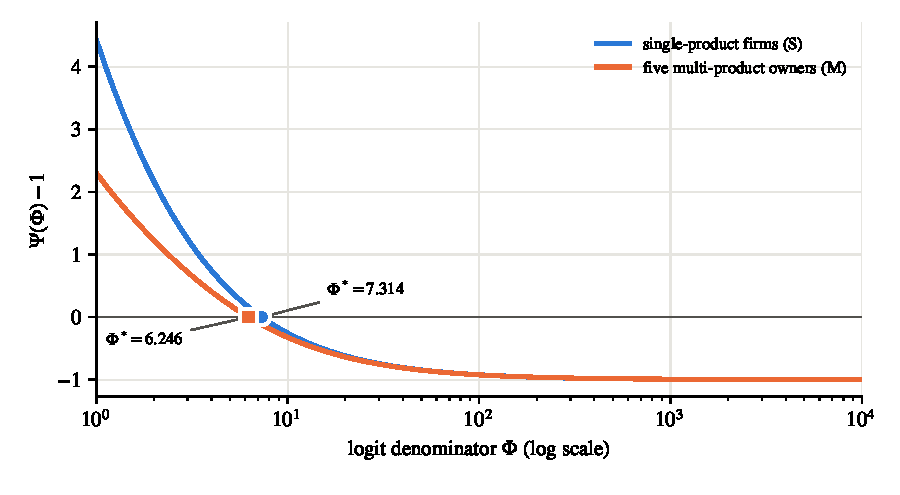
\includegraphics[width=0.82\linewidth]{figures/appC/psi.pdf}
\caption{The aggregate equation \eqref{eq:C-Psi}. Each curve plots $\Psi(\Phi) - 1$, where
$\Psi(\Phi) = \sum_fS_f(\Phi) + \frac{1}{\Phi}$ and $S_f(\Phi)$ solves $S_fe^{\frac{1}{1 - S_f}} = \frac{E_f}{\Phi}$. The curves
are strictly decreasing and cross zero once, at $\Phi^* = \frac{1}{s_0}$. At $\Phi = 1$ they equal 4.44 (S) and
2.31 (M). Computed with \texttt{figures/appC/src/logit\_bertrand.py}.}
\label{fig:C-psi}
\end{figure}

\casehead{Part (g)}
After the merger, owners 3 and 4 form one firm with 13 products, and the other owners are unchanged. Only $\Omega$
changes. \Cref{ex:04-merger-sim} introduces this merger and computes the cost reductions that would offset it. Here we
compare the equilibrium effects with first-round pricing pressure. By \cref{prop:C-unique} the post-merger equilibrium is unique, so the starting point of the iteration does
not matter. Best-response iteration converges in 16 iterations, and the column G of \cref{tab:C-logit-eq} reports the
result.

By \cref{prop:C-common-markup}, the merged firm charges one markup on all 13 products,
$m_M = \frac{1}{\alpha(1 - S_M)} = 0.821$, where $S_M = 39.12$ percent is its post-merger combined share. Before the
merger the markups were 0.636 (owner 3) and 0.670 (owner 4). Every product of owner 3 therefore rises in price by
0.185, and every product of owner 4 by 0.151. The mean increase over the 13 products is 0.167. Rivals respond with
smaller increases: 0.018 for owner 0, 0.013 for owner 2 and 0.004 for owner 1. \Cref{fig:C-logit-merger} plots the
change for every product. Firm-level shares, markups and profits before and after the merger are in
\cref{tab:04-merger-sim}.

The merged firm loses share, from 46.76 to 39.12 percent, and every rival gains. The outside share rises from 16.01
to 18.69 percent, and consumer surplus falls by 0.0773, from 0.9159 to 0.8387. Total profit rises from 0.5261 to
0.5767. The merger is profitable for its parties, whose joint profit rises by 5.0 percent, from 0.3061 to 0.3213.
The rivals gain more in percentage terms: 15.9 percent for owner 0, 16.7 percent for owner 1 and 16.3 percent for
owner 2. Total surplus falls from 1.4421 to 1.4154.

The fall in consumer surplus is an instance of a general result for multi-product logit pricing. A single number
summarizes each firm, its \emph{type}, which is its contribution to consumer surplus if it priced at marginal cost. In
our notation the type of firm $f$ is $E_f$. A merger without cost savings gives the merged firm the type $E_3 + E_4$,
the sum of the partners' types. \citet[Section~3.3.1, p.~229]{AskerNocke2021} report the following result of
\citet{NockeSchutz2019}. Consumer surplus does not fall if and only if the merged type is above a cutoff, which exceeds
the sum of the partners' types. A merger that only combines ownership, like this one, therefore always harms consumers. The aggregative structure behind the result is that of \cref{prop:C-unique}
\citep{NockeSchutz2018}.

\begin{figure}[htbp]
\centering
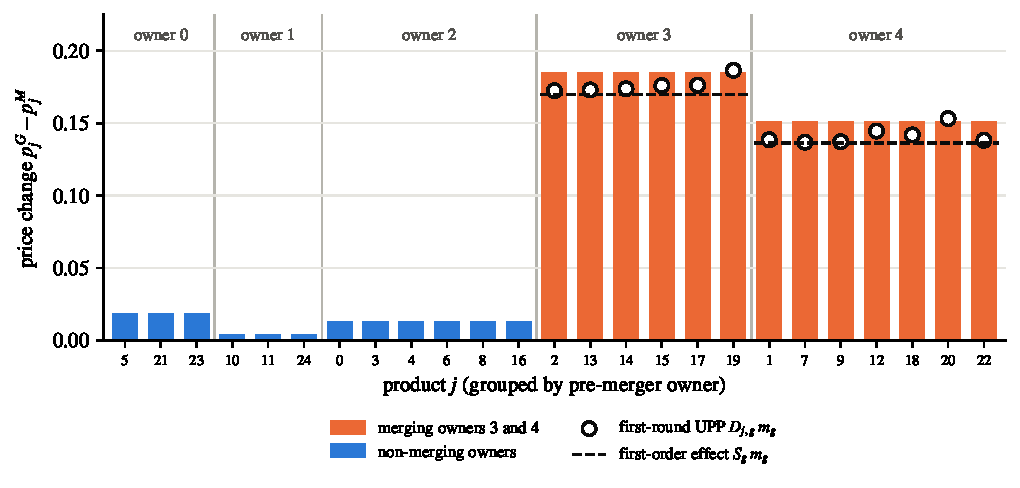
\includegraphics[width=\linewidth]{figures/appC/logit_merger.pdf}
\caption{Price changes caused by the merger of owners 3 and 4, by product. Bars show the change from the
pre-merger equilibrium (M) to the post-merger equilibrium (G). Hollow circles show each merging product's
first-round upward pricing pressure $D_{j,g}m_g$, and dashed lines show the first-order effect $S_gm_g$ of the
firm-level tax. Computed with \texttt{figures/appC/src/logit\_bertrand.py}.}
\label{fig:C-logit-merger}
\end{figure}

\emph{Upward pricing pressure} (UPP) measures the merger's incentive to raise prices at pre-merger prices
(\cref{sec:11-uppfs}). \citet{FarrellShapiro2010} define the first-round tax on product 1 of a merger between two
single-product firms as $t_1 = D_{12}(P_2 - C_2)$, the diversion ratio times the partner's margin (working-paper
version, p.~9). When the partner owns several products, the tax sums over them, $t_j = \sum_kD_{jk}m_k$
(\cref{eq:11-upp-multi}). For product $j$ of owner 3, the partner is owner 4, whose seven products share the
pre-merger markup $m_4$. With logit diversion,
\begin{equation}\label{eq:C-upp-logit}
  \mathit{UPP}_j = \sum_{k \in \mathcal{J}_4}\frac{s_k}{1 - s_j}\,m_4 = \frac{S_4}{1 - s_j}\,m_4 .
\end{equation}
The \emph{gross upward pricing pressure index} (GUPPI) divides by the product's price, $\mathit{GUPPI}_j = \frac{\mathit{UPP}_j}{p_j}$
(\cref{eq:11-guppi}). For owner 3's products, UPP ranges from 0.172 to 0.187 and GUPPI from 0.116 to 0.162. For
owner 4's products, UPP ranges from 0.137 to 0.153 and GUPPI from 0.078 to 0.132
(\cref{tab:C-logit-merger}). The UPP values bracket the equilibrium increases of 0.185 and 0.151 closely.
\citet[Section~3.3.2, pp.~230--231]{AskerNocke2021} present UPP as the simple alternative to full merger simulation.
Simulation estimates demand, recovers marginal costs from an assumption on conduct and solves for the post-merger
equilibrium. Demand and costs are known here, so this part carries out the last step exactly.

\begin{table}[htbp]
\centering
\caption{Pricing pressure and price changes of the merging products}
\label{tab:C-logit-merger}
\footnotesize
\begin{tabular}{@{}lcc@{}}
\toprule
 & Owner 3 (partner $g = 4$) & Owner 4 (partner $g = 3$) \\
\midrule
Product diversion to partner $\frac{S_g}{1 - s_j}$ & 0.257 to 0.278 & 0.215 to 0.241 \\
Product-level UPP $\frac{S_g}{1 - s_j}m_g$ & 0.172 to 0.187 & 0.137 to 0.153 \\
GUPPI $\frac{1}{p_j}\frac{S_g}{1 - s_j}m_g$ & 0.116 to 0.162 & 0.078 to 0.132 \\
Firm-level tax $t_f = \frac{S_gm_g}{1 - S_f}$ & 0.216 & 0.182 \\
First-order effect $(1 - S_f)t_f = S_gm_g$ & 0.170 & 0.136 \\
One round with taxes $t_f$, re-equilibrated & 0.184 & 0.152 \\
Equilibrium price change $m_M - m_f$ & 0.185 & 0.151 \\
\bottomrule
\end{tabular}

\vspace{3pt}
\begin{minipage}{0.97\textwidth}
\footnotesize Notes: Shares and markups are those of the pre-merger equilibrium M, $f$ is the merging owner and $g$
its partner. Ranges are across the owner's products. Firm-level shares, markups and profits before and after the
merger are in \cref{tab:04-merger-sim}. Computed with \texttt{figures/appC/src/logit\_bertrand.py}.
\end{minipage}
\end{table}

Three facts explain why the first-round measure predicts so well here. First, a multi-product firm's internal tax is
a firm-level object. Compare the merged firm's first-order condition for $j \in \mathcal{J}_3$ with owner 3's condition
when each of its products bears a cost increase $t_j$. By \eqref{eq:C-mp-foc} they coincide when
\begin{equation*}
  t_j - \sum_{k \in \mathcal{J}_3}s_kt_k = \sum_{k \in \mathcal{J}_4}s_km_k \qquad \text{for all } j \in \mathcal{J}_3 .
\end{equation*}
With a uniform tax and owner 4's common markup, the solution is $t_3 = \frac{S_4m_4}{1 - S_3}$. In general,
$t_f = \frac{S_gm_g}{1 - S_f}$ for merging firm $f$ with partner $g$. This exceeds the product-level UPP
\eqref{eq:C-upp-logit}, because a joint price increase on all of $f$'s products diverts a larger fraction of sales to
the partner. The firm-level taxes are 0.216 for owner 3 and 0.182 for owner 4.

Second, part (h) shows that a firm passes through a fraction $1 - S_f$ of a uniform cost increase when rivals'
prices are fixed. The first-order price effect is therefore $(1 - S_f)t_f = S_gm_g$, which equals 0.170 for owner 3
and 0.136 for owner 4. Rivals' responses add the rest. Imposing the taxes $t_f$ on owners 3 and 4 and letting all
five owners re-equilibrate gives increases of 0.184 and 0.152, within 0.001 of the merger. Recomputing the taxes at
the new prices and repeating, as Farrell and Shapiro propose, converges to the post-merger equilibrium in nine rounds.
The taxes barely move (owner 3's rises from 0.216 to 0.217), because logit diversion changes little.

Third, an exact decomposition shows the size of the remaining gap. Subtract owner $f$'s pre-merger condition
$m_f = \frac{1}{\alpha} + S_fm_f$ from the merged firm's condition $m_M = \frac{1}{\alpha} + (S_f' + S_g')m_M$, where
primes denote post-merger shares of the former product sets:
\begin{equation}\label{eq:C-merger-decomp}
  m_M - m_f = S_g'\,m_M + \big(S_f'\,m_M - S_f\,m_f\big) .
\end{equation}
For owner 3 the two terms are 0.180 and 0.006, and for owner 4 they are 0.142 and 0.010. The first term exceeds
$S_gm_g$ because the merged markup rises by more (23 and 29 percent) than the partner's share falls (14 and 19
percent). Product-level UPP exceeds $S_gm_g$ by the factor $\frac{1}{1 - s_j}$, between 1.005 and 1.125. The equilibrium
change exceeds $S_gm_g$ by 9 and 11 percent. The closeness of product-level UPP to the equilibrium change thus
reflects two separate corrections of similar size. Imposing the product-level UPP values as taxes, product by
product, would understate the firm's internal tax. Re-equilibrating with them gives increases of only 0.149 and
0.117.

\casehead{Part (h)}
Let all marginal costs rise by a unit tax $t$, so $mc_k(t) = mc_k + t$. Then $v_k(t) = v_k - \alpha t$ and
$E_f(t) = E_fe^{-\alpha t}$ for every firm.

\begin{proposition}[Logit pass-through]\label{prop:C-logit-passthrough}
Let demand be logit with constant marginal costs.
\begin{enumerate}[label=(\roman*)]
  \item Holding rivals' prices fixed, a uniform increase $dc$ in the marginal costs of firm $f$'s products raises
  each of its prices by $(1 - S_f)\,dc$. With one product, the pass-through is $1 - s_j$.
  \item In equilibrium, a common unit tax on all products has pass-through, at $t = 0$,
  \begin{equation}\label{eq:C-tax-pt}
    \rho_f = \frac{dp_k}{dt} = 1 - \frac{S_f\,s_0}{\big[(1 - S_f)^2 + S_f\big]\,(s_0 + \bar w)} \quad (k \in \mathcal{J}_f) ,
    \qquad \bar w = \sum_g\frac{S_g(1 - S_g)^2}{(1 - S_g)^2 + S_g} .
  \end{equation}
  With two or more firms, $1 - S_f < \rho_f < 1$.
\end{enumerate}
\end{proposition}

\begin{proof}
(i) This is \cref{prop:04-passthrough}(iii), and part (i) of that proposition is the single-product case.

(ii) The equilibrium satisfies \eqref{eq:C-h} for every firm and the adding-up condition \eqref{eq:C-Psi}. Since
$\ln h(S) = \ln S + \frac{1}{1 - S}$, differentiating \eqref{eq:C-h} in logarithms gives
\begin{equation*}
  \Big[\frac{1}{S_f} + \frac{1}{(1 - S_f)^2}\Big]dS_f = d\ln E_f - d\ln\Phi = -\alpha\,dt - d\ln\Phi .
\end{equation*}
Write $w_f = \frac{S_f(1 - S_f)^2}{(1 - S_f)^2 + S_f}$, the inverse of the bracket, so that
$dS_f = w_f(-\alpha\,dt - d\ln\Phi)$. Adding up gives $\sum_fdS_f = -d\frac{1}{\Phi} = s_0\,d\ln\Phi$. Summing the
previous equation over firms,
\begin{equation*}
  \bar w\,(-\alpha\,dt - d\ln\Phi) = s_0\,d\ln\Phi
  \quad\Longrightarrow\quad
  d\ln\Phi = -\frac{\alpha\bar w}{s_0 + \bar w}\,dt .
\end{equation*}
Substituting back, $-\alpha\,dt - d\ln\Phi = -\frac{\alpha s_0}{s_0 + \bar w}\,dt$, so
$dS_f = -\frac{\alpha w_fs_0}{s_0 + \bar w}\,dt$. Differentiating \eqref{eq:C-common-markup} then gives
\begin{equation*}
  dm_f = \frac{dS_f}{\alpha(1 - S_f)^2} = -\frac{S_f\,s_0}{\big[(1 - S_f)^2 + S_f\big](s_0 + \bar w)}\,dt ,
\end{equation*}
and $dp_k = dt + dm_f$ gives \eqref{eq:C-tax-pt}. Since $s_0 > 0$, $\rho_f < 1$. For the lower bound, write
$A_f = (1 - S_f)^2 + S_f$, so that $1 - A_f = S_f(1 - S_f)$. Then $\rho_f > 1 - S_f$ holds if and only if
$s_0 < A_f(s_0 + \bar w)$, that is, if and only if $S_f(1 - S_f)\,s_0 < A_f\bar w$. Since $\bar w \ge w_f$, the right
side is at least $A_fw_f = S_f(1 - S_f)^2$. This exceeds $S_f(1 - S_f)s_0$ because $1 - S_f > s_0$ when another firm
has a positive share.
\end{proof}

For a single product, part (i) is also the logit case of \cref{lem:11-passthrough}. Part (ii) gives in closed form, for any ownership structure, the common-tax pass-through
that \cref{cor:04-passthrough-eq} expresses through a matrix inverse for single-product firms. Two special cases help
to read it. Without an outside good ($s_0 \to 0$), a common cost increase is
passed through fully, because relative prices are all that matter. With a single firm, $\bar w = w_f$ and
$s_0 = 1 - S_f$, and \eqref{eq:C-tax-pt} reduces to $\rho_f = 1 - S_f$, the partial pass-through, because no rival
responds. With several firms, the common tax lowers every $E_f$, which by itself cuts $f$'s markup as in part (i). It
also raises rivals' prices, which lowers $\Phi_{-f}$ and offsets part of the fall in $z_f = \frac{E_fe^{-1}}{\Phi_{-f}}$.
Equilibrium pass-through therefore lies between the partial rate and one.

We compute the equilibrium at $t = 0.1$ by best-response iteration and divide each price change by $t$.
\Cref{tab:C-logit-tax} reports the results. Under S, product pass-through ranges from 0.980 to 0.999, with mean
0.994. It is lower for products with larger shares, and its correlation with the share is $-1.000$. Under M it ranges from 0.934 (owner 4) to 0.990 (owner 1),
with mean 0.954. The closed form \eqref{eq:C-tax-pt} at $t = 0$ gives almost the same values, and it matches a
numerical derivative to within $5\times10^{-8}$. Partial pass-through $1 - S_f$ is much lower, down to 0.746 for
owner 4. Rivals' responses account for most of the difference.

\begin{table}[htbp]
\centering
\caption{Pass-through of a common unit tax $t = 0.1$}
\label{tab:C-logit-tax}
\footnotesize
\begin{tabular}{@{}lcc@{}}
\toprule
 & Single-product firms (S) & Multi-product owners (M) \\
\midrule
\multicolumn{3}{@{}l}{\textit{Panel A. Market summary}} \\
Product pass-through at $t = 0.1$: range (mean) & 0.980 to 0.999 (0.994) & 0.934 to 0.990 (0.954) \\
Closed form \eqref{eq:C-tax-pt} at $t = 0$: range & 0.981 to 0.999 & 0.937 to 0.990 \\
Partial pass-through $1 - S_f$: range & 0.883 to 0.996 & 0.746 to 0.953 \\
Pass-through of the share-weighted mean price & 0.9895 & 0.9492 \\
\quad with weights held at pre-tax shares & 0.9893 & 0.9497 \\
\quad composition term & 0.0002 & $-0.0005$ \\
Outside share, before and after & 0.1367, 0.1618 & 0.1601, 0.1873 \\
Consumer surplus, before and after & 0.9949, 0.9107 & 0.9159, 0.8374 \\
Total profit, before and after & 0.4616, 0.4474 & 0.5261, 0.5051 \\
\bottomrule
\end{tabular}

\vspace{6pt}
\begin{tabular}{@{}lccccc@{}}
\toprule
\multicolumn{6}{@{}l}{\textit{Panel B. Owners under M}} \\
Owner & 0 & 1 & 2 & 3 & 4 \\
\midrule
Combined share $S_f$ (\%) & 18.87 & 4.67 & 13.68 & 21.40 & 25.36 \\
Partial pass-through $1 - S_f$ & 0.811 & 0.953 & 0.863 & 0.786 & 0.746 \\
Equilibrium pass-through, closed form at $t = 0$ & 0.955 & 0.990 & 0.969 & 0.949 & 0.937 \\
Equilibrium pass-through at $t = 0.1$ & 0.953 & 0.990 & 0.967 & 0.946 & 0.934 \\
\bottomrule
\end{tabular}

\vspace{3pt}
\begin{minipage}{0.97\textwidth}
\footnotesize Notes: Pass-through at $t = 0.1$ is $\frac{p(0.1) - p(0)}{0.1}$. The composition term is the difference
between the pass-through of the share-weighted mean price and the same object with weights fixed at pre-tax shares.
Computed with \texttt{figures/appC/src/logit\_bertrand.py}.
\end{minipage}
\end{table}

The share-weighted mean price $\bar p = \sum_jw_jp_j$, with $w_j = \frac{s_j}{1 - s_0}$, changes by
\begin{equation*}
  \frac{d\bar p}{dt} = \sum_jw_j\frac{dp_j}{dt} + \sum_jp_j\frac{dw_j}{dt} .
\end{equation*}
The first term is the average product pass-through. The second is a composition term, which is positive when
consumers shift toward expensive products. The mean-price pass-through is 0.9895 under S and 0.9492 under M, and the
composition terms are only 0.0002 and $-0.0005$. A common unit tax shifts all logit prices by similar amounts, so
substitution among inside goods hardly changes the mix.

These results bear on the cigarette tax study of \cref{sec:C-passthrough}. With logit demand and constant marginal
costs, a common tax is passed through less than one for one by every firm, whatever the ownership structure, and
composition effects are negligible. Logit demand is log-concave in own price, which is why pass-through stays below
one. A pass-through rate above one, as \citet{Sumner1981} estimates, needs a feature that this model lacks. Candidates
are demand that is more convex than the logit, composition effects much larger than those found here, or a different
form of conduct.

\subsection{Computational notes}

A single script produces every number in this section. It is \texttt{logit\_bertrand.py} in the folder
\texttt{figures/appC/src}, and it reads the data file \texttt{logit\_market.csv} from the folder
\texttt{figures/appC/data}.
\begin{enumerate}
  \item Compute $a_j = x_j\beta + \xi_j$, $mc_j$ and $v_j = a_j - \alpha\,mc_j$. An owner vector assigns products to
  firms. Under S it is $(0, 1, \dots, 24)$. After the merger, owner 4 is relabeled 3.
  \item For each firm compute $E_f = \sum_{k \in \mathcal{J}_f}e^{v_k}$ once. At each iteration compute
  $\Phi_{-f} = \Phi - \sum_{k \in \mathcal{J}_f}e^{\delta_k}$, the markup \eqref{eq:C-br-multi} with the principal
  branch of $W$, and the new prices.
  \item Stop when the sup-norm change in prices is below $10^{-12}$. Verify \eqref{eq:C-stacked-foc}, the common
  markups \eqref{eq:C-common-markup} and agreement with markup iteration and a root finder.
  \item For uniqueness, solve \eqref{eq:C-h} for $S_f(\Phi)$ in logarithms, $\ln S_f + \frac{1}{1 - S_f} = \ln\frac{E_f}{\Phi}$,
  with a bracketing root finder, and evaluate $\Psi$ on the grid.
  \item For the merger and the tax, re-solve with the new owner vector or with $mc + t$.
\end{enumerate}
The best-response step takes five lines in Python with NumPy and SciPy:
\begin{verbatim}
def best_response(p, owner, mc):
    e = np.exp(a - alpha * p)                                # e^{delta_j}
    E = np.bincount(owner, weights=np.exp(a - alpha * mc))   # E_f
    phi_minus = 1 + e.sum() - np.bincount(owner, weights=e)  # Phi_{-f}
    m = (1 + lambertw(E * np.exp(-1) / phi_minus).real) / alpha
    return mc + m[owner]
\end{verbatim}

\section{Simulating a market with random coefficients demand}\label{sec:C-simulate}

The previous problem computed prices from a known demand system. Empirical work runs in the opposite direction,
from observed prices and shares back to demand and cost. To judge an estimator we need data whose true model we
know. This problem builds such data, and the next three problems use it. We simulate 100 markets
from a random coefficients logit model with multi-product Bertrand pricing, solve for equilibrium prices, and draw the
choices of about ten thousand consumers per market. Sections \ref{sec:C-vertical} to \ref{sec:C-rc-est} estimate the
vertical, logit and random coefficients models on the resulting data. \Cref{sec:08-worked} uses the same design to
illustrate the estimation of the random coefficients model step by step.

\subsection{Statement}

Think of the market for yogurt in 100 metropolitan areas, which we treat as independent markets $t = 0, \dots, 99$.
Ten products exist in total, $j = 1, \dots, 10$. Each market offers between 4 and 9 of them, 6.54 on average, so there
are 654 product-market observations. A product has three characteristics,
$x_{jt} = (1, x^{sug}_{jt}, x^{org}_{jt})$: a constant, its sugar content and an indicator of organic production. Its
marginal cost also depends on a cost shifter $w_{jt}$, the price of milk used in production. Characteristics, the
cost shifter and the owner are fixed by product, so $x_{jt} = x_j$ and $w_{jt} = w_j$ in every market that offers
$j$ (\cref{tab:C-products}). Four firms own the products: firm A owns $\{5, 8\}$, firm B owns $\{1, 4, 6, 7\}$, firm C
owns $\{2, 3, 10\}$ and firm D owns $\{9\}$. Across markets only the set of products offered $\mathcal{J}_t$, the
unobservables $(\xi_{jt}, \omega_{jt})$ and the market size $M_t$ vary. Their values are supplied in the file
\texttt{yogurt\_markets.csv} in the folder \texttt{figures/appC/data}. Market sizes range from 9,756 to 10,223, with
mean 9,998.7.

Consumer $i$ in market $t$ has utility
\begin{equation}\label{eq:C-rc-utility}
  u_{ijt} = \delta_{jt} + \tilde x_{jt}\Sigma\nu_i + \epsilon_{ijt} , \qquad
  \delta_{jt} = x_{jt}\beta - \alpha p_{jt} + \xi_{jt} , \qquad
  u_{i0t} = \epsilon_{i0t} ,
\end{equation}
where $\tilde x_{jt} = (x_{jt}, p_{jt})$ contains the characteristics and the price, $\nu_i \sim N(0, I_4)$, and the
$\epsilon_{ijt}$ are independent type-I extreme value shocks. The parameters are $\beta = (-1, 0.2, 0.15)$,
$\alpha = 3$ and $\Sigma = \diag(\Sigma_{11}, \Sigma_{22}, \Sigma_{33}, \Sigma_{pp}) = \diag(0.5, 0.2, 0.3, 0.5)$.
Marginal cost is
\begin{equation}\label{eq:C-rc-mc}
  mc_{jt} = x_{jt}\gamma_1 + \gamma_2w_{jt} + \omega_{jt} , \qquad \gamma_1 = (0.2, 0.25, 0.3) , \quad \gamma_2 = 0.5 .
\end{equation}
The demand and cost shocks are drawn independently of each other and of the characteristics. Their sample standard
deviations are 0.50 for $\xi_{jt}$ and 0.050 for $\omega_{jt}$, and their sample correlation is 0.004. Firms know all
characteristics, shocks and parameters. Each firm evaluates expected demand by averaging over $n_s = 100$ consumer
types drawn once for each market.

\begin{table}[htbp]
\centering
\caption{Products in the simulated markets}
\label{tab:C-products}
\footnotesize
\begin{tabular}{@{}lcccccccccc@{}}
\toprule
Product $j$ & 1 & 2 & 3 & 4 & 5 & 6 & 7 & 8 & 9 & 10 \\
\midrule
Firm & B & C & C & B & A & B & B & A & D & C \\
Sugar content $x^{sug}_j$ & 1.349 & 1.300 & 0.929 & 1.315 & 1.182 & 0.636 & 1.130 & 1.204 & 1.128 & 0.879 \\
Organic $x^{org}_j$ & 0 & 1 & 0 & 1 & 0 & 0 & 0 & 0 & 1 & 0 \\
Price of milk $w_j$ & 0.534 & 0.367 & 0.426 & 0.547 & 0.346 & 0.529 & 0.588 & 0.334 & 0.527 & 0.442 \\
\midrule
Markets offering $j$ & 77 & 58 & 73 & 65 & 52 & 66 & 66 & 68 & 65 & 64 \\
Mean price & 1.189 & 1.403 & 1.025 & 1.504 & 1.048 & 1.008 & 1.164 & 1.039 & 1.427 & 1.012 \\
Mean markup & 0.390 & 0.395 & 0.381 & 0.402 & 0.378 & 0.384 & 0.390 & 0.376 & 0.378 & 0.382 \\
Mean realized share & 0.015 & 0.010 & 0.024 & 0.009 & 0.023 & 0.024 & 0.019 & 0.027 & 0.011 & 0.024 \\
\bottomrule
\end{tabular}

\vspace{3pt}
\begin{minipage}{0.97\textwidth}
\footnotesize Notes: The first four rows are the design. The last three rows are equilibrium outcomes, averaged over
the markets that offer the product. In the data file the owner codes of firms A, B, C and D are 0, 1, 2 and 4.
Computed with \texttt{figures/appC/src/appC\_simulate.py}.
\end{minipage}
\end{table}

\begin{enumerate}[label=(\alph*)]
  \item Interpret the random coefficients. How likely is a consumer to like higher prices?
  \item Write the expected-share function that the firms use, with $n_s = 100$ fixed draws per market, and explain how
  to evaluate it without numerical overflow.
  \item Derive the first-order conditions of multi-product Bertrand pricing and an algorithm that solves them. Solve
  every market and check the solutions.
  \item Simulate the realized shares of $M_t$ consumers per market and compare them with the expected shares.
  \item Report the equilibrium of market 0.
  \item Show that, when individual choice probabilities are small, the markup of product $j$ is close to the inverse
  of the average price sensitivity of its buyers. Evaluate the approximation in market 0.
  \item Derive the sampling error of a realized share and of its logarithm, and evaluate it in market 0.
\end{enumerate}

\subsection{Solution}

\casehead{Part (a)}
Because $\Sigma$ is diagonal, the consumer-specific term in \eqref{eq:C-rc-utility} is
\begin{equation*}
  \tilde x_{jt}\Sigma\nu_i = 0.5\,\nu_{i1} + 0.2\,\nu_{i2}x^{sug}_{jt} + 0.3\,\nu_{i3}x^{org}_{jt} + 0.5\,\nu_{i4}p_{jt} .
\end{equation*}
Consumer $i$ therefore has her own coefficients
\begin{equation}\label{eq:C-rc-coefs}
  \beta_{i1} = -1 + 0.5\,\nu_{i1} , \quad \beta_{i2} = 0.2 + 0.2\,\nu_{i2} , \quad
  \beta_{i3} = 0.15 + 0.3\,\nu_{i3} , \quad -\alpha_i \text{ with } \alpha_i = 3 - 0.5\,\nu_{i4} .
\end{equation}
The random constant $\beta_{i1}$ shifts the utility of every inside good relative to the outside good. Consumers
who like yogurt are more likely to buy some yogurt. Inside goods therefore substitute more with one another than
with the outside good, as in a nested logit with one nest of inside goods. The coefficients on sugar and on organic
production are positive on average, but 15.9 percent of consumers dislike sugar ($\nu_{i2} < -1$) and 30.9 percent
dislike organic production ($\nu_{i3} < -0.5$). The price sensitivity $\alpha_i$ is normal with mean 3 and standard
deviation 0.5. A consumer likes higher prices only if $\alpha_i \le 0$, that is, if $\nu_{i4} \ge 6$. This has
probability $\Pr(\nu_{i4} \ge 6) = 9.9\times10^{-10}$. Among the 10,000 consumer types the firms use, $\alpha_i$
ranges from 1.17 to 4.79.

Conditional on $\nu_i$, the extreme value shocks give logit choice probabilities. With
$V_{ijt} = \delta_{jt} + \tilde x_{jt}\Sigma\nu_i$,
\begin{equation}\label{eq:C-rc-sij}
  s_{ijt} = \frac{e^{V_{ijt}}}{1 + \sum_{k \in \mathcal{J}_t}e^{V_{ikt}}} , \qquad
  s_{jt} = \int_{\R^4} s_{ijt}(\nu)\,\phi_4(\nu)\,\dd\nu ,
\end{equation}
where $s_{ijt}(\nu)$ is the choice probability of a consumer with taste vector $\nu$ and $\phi_4$ is the
four-dimensional standard normal density. The integral breaks the
independence of irrelevant alternatives. A rise in $p_{kt}$ moves consumers who were likely to buy $k$, and these
consumers are most likely to buy products similar to $k$ (\cref{prop:08-derivs}). Cross elasticities therefore vary
across products, unlike \eqref{eq:C-logit-elast}.

\casehead{Part (b)}
For each market we draw $n_s = 100$ vectors $\nu_{it} \sim N(0, I_4)$ once and keep them fixed. They are the consumer
types whose average demand the firms compute. The expected share of product $j$ is the simulator of
\citet[eq.~11, p.~532]{Nevo2000a},
\begin{equation}\label{eq:C-rc-simshare}
  s_{jt}(p_t) = \frac{1}{n_s}\sum_{i=1}^{n_s}s_{ijt}(p_t) , \qquad
  s_{ijt}(p_t) = \frac{e^{V_{ijt}}}{1 + \sum_{k \in \mathcal{J}_t}e^{V_{ikt}}} .
\end{equation}
Prices enter twice, through $\delta_{jt}$ and through the last element of $\tilde x_{jt}$, so the function must rebuild
$\tilde x_{jt}$ whenever prices change.

Exponentials overflow when utilities are large. For draw $i$, let $c_i = \max\{0, \max_kV_{ikt}\}$, where the 0 is the
outside good's utility. Multiplying the numerator and the denominator of $s_{ijt}$ by $e^{-c_i}$ gives
\begin{equation*}
  s_{ijt} = \frac{e^{V_{ijt} - c_i}}{e^{-c_i} + \sum_{k \in \mathcal{J}_t}e^{V_{ikt} - c_i}} .
\end{equation*}
The value is unchanged. Every exponent is now at most zero, so nothing overflows, and the largest term in the
denominator equals one, so the denominator cannot underflow to zero.

The draws stay fixed for two reasons. With fixed draws, $s_t(p_t)$ is a smooth deterministic function of prices, so the
first-order conditions of part (c) define a well-posed system. With fresh draws at each evaluation, the system would
change from one iteration to the next, and no solver could converge. In this design the 100 draws also define what
firms believe about demand. Part (d) shows that these beliefs differ from population demand by simulation error.

\casehead{Part (c)}
Firm $f$ owns the products $\mathcal{J}_{ft} \subseteq \mathcal{J}_t$ and earns
$\pi_{ft} = M_t\sum_{k \in \mathcal{J}_{ft}}(p_{kt} - mc_{kt})s_{kt}(p_t)$. Market size multiplies profit, so it drops out of
the first-order conditions
\begin{equation}\label{eq:C-rc-foc}
  s_{jt} + \sum_{k \in \mathcal{J}_{ft}}(p_{kt} - mc_{kt})\frac{\partial s_{kt}}{\partial p_{jt}} = 0 , \qquad j \in \mathcal{J}_{ft} .
\end{equation}
These are equations (3.3) of \citet[p.~853]{BerryLevinsohnPakes1995}. For draw $i$, price enters $V_{ijt}$ with
coefficient $\frac{\partial V_{ijt}}{\partial p_{jt}} = -\alpha + 0.5\,\nu_{i4} = -\alpha_i$. The quotient rule of
\cref{sec:C-logit-bertrand}, applied draw by draw, gives
$\frac{\partial s_{ijt}}{\partial p_{kt}} = \alpha_is_{ijt}(s_{ikt} - \indic\{j = k\})$. Averaging over draws,
\begin{equation}\label{eq:C-rc-deriv}
  \Delta_{jk,t} = \frac{\partial s_{jt}}{\partial p_{kt}} = \frac{1}{n_s}\sum_{i=1}^{n_s}\alpha_is_{ijt}\big(s_{ikt} - \indic\{j = k\}\big) .
\end{equation}
With $\Omega_t$ the ownership matrix of market $t$, the conditions stack as in \eqref{eq:C-stacked-foc}:
$s_t + (\Omega_t \odot \Delta_t^\top)(p_t - mc_t) = 0$. Solving for the markups gives
$p_t - mc_t = -(\Omega_t \odot \Delta_t^\top)^{-1}s_t$, which is equation (3.5) of
\citet[p.~854]{BerryLevinsohnPakes1995} with their matrix equal to $-(\Omega_t \odot \Delta_t^\top)$.

\begin{proposition}[Morrow-Skerlos fixed point]\label{prop:C-ms}
Let $\Lambda_t$ be the diagonal matrix with $\Lambda_{jj,t} = \frac{1}{n_s}\sum_i\alpha_is_{ijt}$, and let $\Gamma_t$ be
the matrix with $\Gamma_{jk,t} = \frac{1}{n_s}\sum_i\alpha_is_{ijt}s_{ikt}$. If every $\alpha_i > 0$, the first-order
conditions hold at $p_t$ if and only if
\begin{equation}\label{eq:C-ms-zeta}
  p_t - mc_t = \zeta_t(p_t) \equiv \Lambda_t^{-1}\big[s_t + (\Omega_t \odot \Gamma_t)(p_t - mc_t)\big] ,
\end{equation}
where $\Lambda_t$, $\Gamma_t$ and $s_t$ are evaluated at $p_t$.
\end{proposition}

\begin{proof}
By \eqref{eq:C-rc-deriv}, $\Delta_t = -\Lambda_t + \Gamma_t$, and $\Gamma_t$ is symmetric. Since $\Omega_t$ is symmetric
with a unit diagonal, $\Omega_t \odot \Lambda_t = \Lambda_t$, and
\begin{equation*}
  (\Omega_t \odot \Delta_t)^\top = -\Lambda_t + \Omega_t \odot \Gamma_t .
\end{equation*}
The first-order conditions therefore read $s_t - \Lambda_t(p_t - mc_t) + (\Omega_t \odot \Gamma_t)(p_t - mc_t) = 0$.
Every diagonal entry of $\Lambda_t$ is positive because $\alpha_i > 0$ and $s_{ijt} > 0$. Moving the $\Lambda_t$ term
to the left and multiplying by $\Lambda_t^{-1}$ gives \eqref{eq:C-ms-zeta}. Each step is reversible.
\end{proof}

This is \cref{prop:08-ms}, due to \citet{MorrowSkerlos2011}. In the plain logit, $\alpha_i = \alpha$ gives
$\Lambda_{jj} = \alpha s_j$ and $\Gamma_{jk} = \alpha s_js_k$, and \eqref{eq:C-ms-zeta} becomes
$m_j = \frac{1}{\alpha} + \sum_{k \in \mathcal{J}_f}s_km_k$, the multi-product condition \eqref{eq:C-mp-foc}. Here every
$\alpha_i$ exceeds 1.17, so the proposition applies. We solve each market as follows.
\begin{enumerate}
  \item Start at $p_t^{(0)} = mc_t$.
  \item Given $p_t^{(n)}$, compute $s_{ijt}$ for the 100 draws, then $s_t$, $\Lambda_t$ and $\Gamma_t$.
  \item Set $p_t^{(n+1)} = mc_t + \zeta_t(p_t^{(n)})$.
  \item Stop when $\|p_t^{(n+1)} - p_t^{(n)}\|_\infty < 10^{-12}$. Otherwise return to step 2.
  \item Verify the first-order conditions \eqref{eq:C-rc-foc} at the solution.
\end{enumerate}
Nothing guarantees that $p \mapsto mc + \zeta(p)$ is a contraction, so convergence must be checked market by market.

\Cref{tab:C-sim-checks} reports the diagnostics. The iteration converges in every market, in 10 to 13 iterations
(11.05 on average). The largest first-order residual across markets is $8.6\times10^{-15}$. A hybrid Powell root finder
on \eqref{eq:C-rc-foc}, started at marginal cost, reaches the same prices to within $1.0\times10^{-13}$. We then restart
from 20 random price vectors per market, with each price drawn uniformly on $[0, 4]$. All 2,000 runs of the
iteration return the original prices, to within $2.1\times10^{-13}$, so no market shows a second equilibrium.

The root finder is less reliable from the random starts. Applied to the residual of \eqref{eq:C-rc-foc}, it solves
only 13 of the 2,000 problems. Every term of that residual tends to zero as prices rise without bound. The root
finder can therefore stop at very high prices, where the residual is small and no equilibrium is near. Applied to the residual
$\zeta_t(p) - (p - mc_t)$, which is measured in price units, it solves 1,817 of the 2,000 problems, and every
solution it finds is the original one.

Equilibrium prices range from 0.881 to 1.609, with mean 1.180. Markups range from 0.348 to 0.451, with mean 0.386,
and the Lerner index averages 0.334. Markups are close to the inverse of the mean price coefficient,
$\frac{1}{3} = 0.333$, for a reason that part (f) makes precise.

\begin{table}[htbp]
\centering
\caption{Simulated markets: equilibrium computation and realized shares}
\label{tab:C-sim-checks}
\footnotesize
\begin{tabular}{@{}lr@{}}
\toprule
\multicolumn{2}{@{}l}{\textit{Panel A. Equilibrium prices}} \\
Morrow-Skerlos iterations per market, range (mean) & 10 to 13 (11.05) \\
Largest first-order residual & $8.6\times10^{-15}$ \\
Largest price difference, iteration versus root finder & $1.0\times10^{-13}$ \\
Random restarts solved by the iteration, largest deviation & 2,000 of 2,000, $2.1\times10^{-13}$ \\
Random restarts solved by a root finder on \eqref{eq:C-rc-foc} & 13 of 2,000 \\
Random restarts solved by a root finder on $\zeta_t(p) - (p - mc_t)$ & 1,817 of 2,000 \\
Markets with a second equilibrium & 0 \\
Prices: range (mean) & 0.881 to 1.609 (1.180) \\
Markups: range (mean) & 0.348 to 0.451 (0.386) \\
Lerner index: range (mean) & 0.234 to 0.448 (0.334) \\
\midrule
\multicolumn{2}{@{}l}{\textit{Panel B. Realized shares}} \\
Simulated consumers & 999,870 \\
Products with zero realized share & 0 \\
Smallest realized share (buyers) & 0.0019 (19) \\
Mean and largest absolute gap, realized minus expected share & 0.0014, 0.0100 \\
Correlation of realized and expected shares & 0.986 \\
Outside share: mean (range across markets) & 0.879 (0.788 to 0.948) \\
Mean squared standardized gap: realized minus population share & 1.07 \\
Mean squared standardized gap: expected minus population share & 0.84 \\
Mean squared standardized gap: realized minus expected share & 1.88 \\
\bottomrule
\end{tabular}

\vspace{3pt}
\begin{minipage}{0.97\textwidth}
\footnotesize Notes: 654 product-market observations in 100 markets. Random restarts draw each starting price from
$U[0, 4]$, 20 per market. A run counts as solved when the largest markup residual is below $10^{-10}$. Standardized
gaps divide by the sampling standard deviation $\sqrt{\frac{s(1 - s)}{M_t}}$, where $s$ is the population share
computed with 100,000 draws. Computed with \texttt{figures/appC/src/appC\_simulate.py}.
\end{minipage}
\end{table}

\casehead{Part (d)}
At the equilibrium prices we simulate the choices of $M_t$ consumers in each market. Each consumer receives a fresh
draw $\nu_i \sim N(0, I_4)$ and $|\mathcal{J}_t| + 1$ fresh extreme value shocks, one for each product and one for the
outside good. She chooses the alternative with the highest utility $u_{ijt}$. The \emph{realized share} of product $j$
is the fraction of consumers who choose it,
\begin{equation}\label{eq:C-realized}
  \hat s_{jt} = \frac{q_{jt}}{M_t} , \qquad q_{jt} = \sum_{i=1}^{M_t}\indic\Big\{j = \argmax_{k \in \mathcal{J}_t \cup \{0\}}u_{ikt}\Big\} .
\end{equation}
Realized shares, prices, characteristics, the cost shifter and ownership are the data that Sections
\ref{sec:C-vertical} to \ref{sec:C-rc-est} use. The unobservables, the marginal costs and the expected shares are
kept only to evaluate the estimators.

In total we simulate 999,870 consumers. No product has a zero realized share, and the smallest realized share is
0.0019, or 19 buyers. The mean absolute difference between realized and expected shares is 0.0014, the largest is
0.0100, and their correlation is 0.986. The outside good is large. Its realized share averages 0.879 across markets
and ranges from 0.788 to 0.948.

Three share concepts are at work. The expected share $s_{jt}$ averages over the firms' 100 draws. The
\emph{population share} $s^\infty_{jt}$ integrates over the whole normal distribution, and we approximate it with
100,000 draws per market. The realized share $\hat s_{jt}$ is a sample proportion among $M_t$ consumers drawn from the
population. The gap between realized and expected shares therefore has two parts,
\begin{equation*}
  \hat s_{jt} - s_{jt} = \big(\hat s_{jt} - s^\infty_{jt}\big) + \big(s^\infty_{jt} - s_{jt}\big) ,
\end{equation*}
\emph{sampling error} from the finite number of consumers and \emph{simulation error} from the finite number of firm
draws. Part (g) shows that the sampling error has standard deviation close to $\sqrt{\frac{s(1 - s)}{M_t}}$. Dividing
each part by this standard deviation and averaging the squares over the 654 observations gives 1.07 for the sampling
part, close to the value of one that the binomial formula predicts. It gives 0.84 for the simulation part, and 1.88
for the total. With $n_s = 100$, the firms' simulation error is about as large as the sampling error of
ten thousand consumers. The median relative simulation error $|\frac{s_{jt}}{s^\infty_{jt}} - 1|$ is 4.7 percent, and
the largest is 29 percent.

\casehead{Part (e)}
\Cref{tab:C-mkt0} reports market 0, which offers products 2, 3, 4, 6, 8, 9 and 10 and has $M_0 = 9{,}880$ consumers.
Markups lie between 0.375 and 0.400. The Lerner index ranges from 0.260 for product 9, the most expensive product, to
0.408 for product 10, the cheapest. The outside good's expected share is 0.8463 and its realized share is 0.8549.
Realized and expected shares are close. The largest relative gaps are $-20$ percent for product 9 and $-11$ percent
for product 10. In market 0 the firms' 100 draws overstate demand for every inside product. The expected shares
exceed the population shares by 4 to 10 percent, and the population outside share is 0.8555.

\begin{table}[htbp]
\centering
\caption{Equilibrium in market 0 and the anatomy of its markups}
\label{tab:C-mkt0}
\footnotesize
\setlength{\tabcolsep}{4.5pt}
\begin{tabular}{@{}lcccccccccc@{}}
\toprule
 & & & & & \multicolumn{3}{c}{Share} & & & \\
\cmidrule(lr){6-8}
Product & Firm & $mc_j$ & $p_j$ & $m_j$ & Expected & Realized & Population & Buyers $q_j$ & $\frac{1}{\bar\alpha_j}$ & $\Gamma$ term \\
\midrule
2 & C & 0.9204 & 1.3200 & 0.3995 & 0.0048 & 0.0052 & 0.0044 & 51 & 0.3669 & 0.0326 \\
3 & C & 0.6308 & 1.0182 & 0.3874 & 0.0272 & 0.0252 & 0.0259 & 249 & 0.3584 & 0.0290 \\
4 & B & 1.0286 & 1.4196 & 0.3910 & 0.0125 & 0.0126 & 0.0113 & 124 & 0.3703 & 0.0207 \\
6 & B & 0.6238 & 0.9993 & 0.3755 & 0.0200 & 0.0203 & 0.0192 & 201 & 0.3583 & 0.0172 \\
8 & A & 0.7291 & 1.1246 & 0.3955 & 0.0593 & 0.0560 & 0.0556 & 553 & 0.3616 & 0.0339 \\
9 & D & 1.0729 & 1.4497 & 0.3768 & 0.0072 & 0.0058 & 0.0066 & 57 & 0.3717 & 0.0051 \\
10 & C & 0.5585 & 0.9429 & 0.3845 & 0.0226 & 0.0201 & 0.0215 & 199 & 0.3559 & 0.0285 \\
\midrule
Outside good & & & & & 0.8463 & 0.8549 & 0.8555 & 8,446 & & \\
\bottomrule
\end{tabular}

\vspace{3pt}
\begin{minipage}{0.97\textwidth}
\footnotesize Notes: $M_0 = 9{,}880$. Expected shares average over the firms' 100 draws, population shares over
100,000 draws, and realized shares are fractions of the $M_0$ simulated consumers. $\bar\alpha_j$ is the mean price
sensitivity of product $j$'s buyers among the firms' draws, and the $\Gamma$ term is the second term of
\eqref{eq:C-markup-decomp}, so $m_j = \frac{1}{\bar\alpha_j} + \Gamma$ term. Computed with
\texttt{figures/appC/src/appC\_simulate.py}.
\end{minipage}
\end{table}

\casehead{Part (f)}
Rewrite \eqref{eq:C-ms-zeta} product by product. Dividing the $j$-th row by $\Lambda_{jj}$ gives the exact decomposition
\begin{equation}\label{eq:C-markup-decomp}
  m_j = \frac{s_j}{\Lambda_{jj}} + \frac{1}{\Lambda_{jj}}\sum_{k \in \mathcal{J}_f}\Gamma_{jk}m_k .
\end{equation}

\begin{proposition}[Markups and the price sensitivity of buyers]\label{prop:C-buyer-alpha}
Suppose every $\alpha_i > 0$. Let $\bar\alpha_j = \frac{\Lambda_{jj}}{s_j}$.
\begin{enumerate}[label=(\roman*)]
  \item $\bar\alpha_j$ is the mean price sensitivity of product $j$'s buyers,
  \begin{equation}\label{eq:C-buyer-alpha}
    \bar\alpha_j = \frac{\sum_i\alpha_is_{ij}}{\sum_is_{ij}} = \E\big[\alpha_i \mid i \text{ buys } j\big] ,
  \end{equation}
  where the expectation is over the $n_s$ consumer types and their extreme value shocks.
  \item The markup satisfies
  \begin{equation}\label{eq:C-buyer-bound}
    \Big|m_j - \frac{1}{\bar\alpha_j}\Big| \le \Big(\max_{k \in \mathcal{J}_f}|m_k|\Big)\sum_{k \in \mathcal{J}_f}\max_is_{ik} .
  \end{equation}
  Hence $m_j$ approaches $\frac{1}{\bar\alpha_j}$ as the individual choice probabilities of firm $f$'s products tend to
  zero.
\end{enumerate}
\end{proposition}

\begin{proof}
(i) Each type is equally likely, with probability $\frac{1}{n_s}$, and type $i$ buys $j$ with probability $s_{ij}$. By
Bayes' rule, the probability that a buyer of $j$ is of type $i$ is $\frac{s_{ij}}{\sum_{i'}s_{i'j}}$. Averaging
$\alpha_i$ with these weights gives \eqref{eq:C-buyer-alpha}, and the factor $\frac{1}{n_s}$ cancels from
$\frac{\Lambda_{jj}}{s_j}$.

(ii) By \eqref{eq:C-markup-decomp}, $m_j - \frac{1}{\bar\alpha_j} = \sum_{k \in \mathcal{J}_f}\frac{\Gamma_{jk}}{\Lambda_{jj}}m_k$.
Each ratio is a weighted average of $s_{ik}$ over types, with non-negative weights $\alpha_is_{ij}$:
\begin{equation*}
  \frac{\Gamma_{jk}}{\Lambda_{jj}} = \frac{\sum_i\alpha_is_{ij}\,s_{ik}}{\sum_i\alpha_is_{ij}} \le \max_is_{ik} .
\end{equation*}
The triangle inequality gives \eqref{eq:C-buyer-bound}.
\end{proof}

The markup is thus the inverse of the buyers' mean price sensitivity, corrected by a term of the order of the
firm's individual choice probabilities. This is the discrete-choice form of the inverse semi-elasticity rule
(\cref{eq:08-ms-approx}). In the plain logit, $\bar\alpha_j = \alpha$ for every product, which is why all markups in
\cref{sec:C-logit-bertrand} lie near $\frac{1}{\alpha}$. With random coefficients, buyers select themselves. Consumers
with high $\alpha_i$ buy the outside good more often, so the buyers of any inside product are less price sensitive
than the population.

\Cref{tab:C-mkt0} evaluates the decomposition in market 0. The mean of $\alpha_i$ over the firms' 100 draws is 3.028,
and the mean among consumers who choose the outside good is 3.075. The buyers' mean sensitivity $\bar\alpha_j$ ranges
from 2.690 (product 9) to 2.810 (product 10). Its inverse lies between 0.356 and 0.372 and accounts for 91 to 99
percent of each markup. The expensive organic products 9 and 4 attract the least price-sensitive buyers, with
$\bar\alpha_j$ of 2.690 and 2.701. The $\Gamma$ term accounts for the rest, between 1.4 and 8.6 percent of the markup.
It has two parts. The diagonal part restores the factor $1 - s_{ij}$ in each type's own-price derivative and is
largest for product 8 (0.034), the product with the largest share. The off-diagonal part is the value of sales
recaptured by the firm's other products and is largest for firm C's product 2 (0.029). Firm D sells one product, so
product 9 has no recapture. Product 2 carries the highest markup in the market, 0.3995, although its buyers are more
price sensitive than those of products 4 and 9. Firm C's recapture of 0.029 lifts it to the top. Net of the recapture
terms, product 2's markup is 0.370, the fifth highest of the seven.

\casehead{Part (g)}
Given prices, the $M_t$ consumers choose independently, and each chooses $j$ with probability $s^\infty_{jt}$. Hence
$q_{jt}$ is binomial with parameters $M_t$ and $s^\infty_{jt}$. Writing $s$ for $s^\infty_{jt}$,
\begin{equation}\label{eq:C-share-var}
  \E[\hat s_{jt}] = s , \qquad \Var(\hat s_{jt}) = \frac{s(1 - s)}{M_t} .
\end{equation}
The inversions in Sections \ref{sec:C-vertical} to \ref{sec:C-rc-est} use logarithms of shares. A first-order Taylor
expansion, $\ln\hat s_{jt} \approx \ln s + \frac{\hat s_{jt} - s}{s}$, gives the delta-method variance
(\cref{app:econometrics}),
\begin{equation}\label{eq:C-logshare-var}
  \Var(\ln\hat s_{jt}) \approx \frac{1 - s}{M_ts} = \frac{1 - s}{\E[q_{jt}]} .
\end{equation}
The standard error of a log share is about one over the square root of the number of buyers. A second-order expansion
gives the bias $\E[\ln\hat s_{jt}] - \ln s \approx -\frac{\Var(\hat s_{jt})}{2s^2} = -\frac{1 - s}{2M_ts}$, the
sampling analogue of the simulation bias in \cref{prop:08-simbias}. The logit inversion of \cref{ch:logit} uses the
difference $\ln\hat s_{jt} - \ln\hat s_{0t}$. Since $\Cov(\hat s_{jt}, \hat s_{0t}) = -\frac{s_{jt}s_{0t}}{M_t}$, the
delta method gives $\Cov(\ln\hat s_{jt}, \ln\hat s_{0t}) \approx -\frac{1}{M_t}$, and
\begin{equation}\label{eq:C-logratio-var}
  \Var\Big(\ln\frac{\hat s_{jt}}{\hat s_{0t}}\Big)
  \approx \frac{1 - s_{jt}}{M_ts_{jt}} + \frac{1 - s_{0t}}{M_ts_{0t}} + \frac{2}{M_t}
  = \frac{1}{M_ts_{jt}} + \frac{1}{M_ts_{0t}} .
\end{equation}
The variance is the sum of the inverse expected counts of the two alternatives.

In market 0, product 2 has 51 buyers and product 8 has 553. We evaluate \eqref{eq:C-logshare-var} at the realized
shares. The standard error of the log share is 0.140 for product 2, 0.132 for product 9 and 0.089 for product 4. It
is 0.070 for products 6 and 10, 0.063 for product 3 and 0.041 for product 8. Across all 654 observations the standard error ranges from 0.032
to 0.229, with median 0.080, and 162 observations have fewer than 100 buyers. These errors are small relative to the
standard deviation of $\xi_{jt}$, which is 0.50. They enter the dependent variable of every inversion in Sections
\ref{sec:C-vertical} to \ref{sec:C-rc-est}. To first order they have mean zero and are independent of the instruments,
so they add noise without biasing linear instrumental variable estimators. The second-order bias is largest for the
smallest products, about $-0.010$ for product 2.

\subsection{Computational notes}

A single script produces the data and every number in this section. It is \texttt{appC\_simulate.py} in the folder
\texttt{figures/appC/src}, and it reads the data file \texttt{yogurt\_markets.csv} from the folder
\texttt{figures/appC/data}. The file holds characteristics, the cost shifter, owners, $(\xi_{jt}, \omega_{jt})$ and
$M_t$. The script runs in about two minutes.
\begin{enumerate}
  \item Sort observations by market and product. Compute $mc_{jt}$ from \eqref{eq:C-rc-mc}.
  \item Draw the firms' consumer types in one call, an array of shape $100 \times 100 \times 4$ with seed 2026, markets
  in increasing order. Save it as \texttt{figures/appC/data/firm\_draws.npz}.
  \item In each market, solve \eqref{eq:C-ms-zeta} from $p = mc$, check it with the root finder, and restart from 20 random
  price vectors (seed 2028).
  \item Simulate $M_t$ consumers at the equilibrium prices (seed 2027) and record the counts $q_{jt}$. Compute population
  shares with 100,000 draws per market (seed 2029).
  \item Write \texttt{figures/appC/data/simulated\_market.csv}, with one row per product and market. Its columns are
  the market and product identifiers, owner, characteristics, milk price, market size, price, expected and realized
  shares and the number of buyers. They also hold the true marginal cost, $\xi_{jt}$, $\omega_{jt}$ and $\delta_{jt}$.
\end{enumerate}
The core of the iteration takes two lines once $s_t$, $\Lambda_t$ and $\Gamma_t$ are computed:
\begin{verbatim}
s, lam, gam = share_moments(p)          # s_t, diag(Lambda_t), Gamma_t
p_new = mc + (s + (own * gam.T) @ (p - mc)) / lam
\end{verbatim}
Here \texttt{own} is $\Omega_t$ and \texttt{lam} holds the diagonal of $\Lambda_t$.
